\documentclass[]{fairmeta}
% Option "twocolumn" available, but please prioritize single-column

\usepackage{wrapfig}
\usepackage{tabularx}

\def\vx{{\bm{x}}}

\newlength\savewidth\newcommand\shline{\noalign{\global\savewidth\arrayrulewidth \global\arrayrulewidth 1pt}\hline\noalign{\global\arrayrulewidth\savewidth}}
\newcommand{\tablestyle}[2]{\setlength{\tabcolsep}{#1}\renewcommand{\arraystretch}{#2}\centering\footnotesize}

\newcolumntype{x}[1]{>{\centering\arraybackslash}p{#1pt}}
\newcolumntype{y}[1]{>{\raggedright\arraybackslash}p{#1pt}}
\newcolumntype{z}[1]{>{\raggedleft\arraybackslash}p{#1pt}}

\setlength{\abovecaptionskip}{1pt}

\renewcommand{\paragraph}[1]{\vspace{1.25mm}\noindent\textbf{#1}}

\usepackage{algorithm}
\usepackage{listings}
% \usepackage{lmodern}

\definecolor{codeblue}{rgb}{0.25, 0.5, 0.5}
\definecolor{codekw}{rgb}{0.35, 0.35, 0.75}
\lstdefinestyle{Pytorch}{
    language = Python,
    backgroundcolor = \color{white},
    basicstyle = \fontsize{9pt}{8pt}\selectfont\ttfamily\bfseries,
    columns = fullflexible,
    aboveskip=1pt,
    belowskip=1pt,
    breaklines = true,
    captionpos = b,
    commentstyle = \color{codeblue},
    keywordstyle = \color{codekw},
}

% \definecolor{codeblue}{rgb}{0.25, 0.5, 0.5}
% \definecolor{codekw}{rgb}{0.35, 0.35, 0.75}
% \lstdefinestyle{Pytorch}{
%     language         = Python,
%     backgroundcolor  = \color{white},
%     basicstyle = \fontsize{8.0pt}{9pt}\selectfont\ttfamily\bfseries,
%     columns          = fullflexible,
%     breaklines       = true,
%     captionpos       = b,
%     commentstyle     = \fontsize{4pt}{4pt}\color{codeblue},
%     keywordstyle     = \fontsize{4pt}{4pt}\color{codekw},
%     morekeywords     = {with,scatter_,norm,sort},
% }

\definecolor{green}{HTML}{009000}
\definecolor{red}{HTML}{ea4335}
\newcommand{\better}[1]{\textcolor{green}{$\uparrow\,$#1}}
\newcommand{\worse}[1]{\textcolor{red}{$\downarrow\,$#1}}
\newcommand{\betterinv}[1]{\textcolor{green}{$\downarrow\,$#1}}
\newcommand{\worseinv}[1]{\textcolor{red}{$\uparrow\,$#1}}


\title{Transformers without Normalization}

\author[1,2]{Jiachen Zhu}
\author[1]{Xinlei Chen}
\author[3]{Kaiming He}
\author[1,2]{Yann LeCun}
\author[1,4,\dagger]{Zhuang Liu}


\affiliation[1]{FAIR, Meta}
\affiliation[2]{New York University}
\affiliation[3]{MIT}
\affiliation[4]{Princeton University}
\contribution[\dagger]{Project lead}

\abstract{
Normalization layers are ubiquitous in modern neural networks and have long been considered essential.
This work demonstrates that Transformers without normalization can achieve the same or better performance using a remarkably simple technique.
We introduce Dynamic Tanh (DyT), an element-wise operation $\mathrm{DyT}(\vx) = \tanh(\alpha \vx)$, as a drop-in replacement for normalization layers in Transformers.
DyT is inspired by the observation that layer normalization in Transformers often produces tanh-like, $S$-shaped input-output mappings.
By incorporating DyT, Transformers without normalization can match or exceed the performance of their normalized counterparts, mostly without hyperparameter tuning.
We validate the effectiveness of Transformers with DyT across diverse settings, ranging from recognition to generation, supervised to self-supervised learning, and computer vision to language models.
These findings challenge the conventional understanding that normalization layers are indispensable in modern neural networks, and offer new insights into their role in deep networks.
}

\date{\today} 
\metadata[Project page and code]{{\href{https://jiachenzhu.github.io/DyT}{\texttt{jiachenzhu.github.io/DyT}}}}
\metadata[Correspondence]{\email{jiachen.zhu@nyu.edu}, \email{zhuangl@princeton.edu}}
% {\href{https://github.com/jiachenzhu/DyT}{\texttt{github.com/jiachenzhu/DyT}}, 
\begin{document}

\maketitle

% CVPR 2025 Paper Template; see https://github.com/cvpr-org/author-kit

\documentclass[10pt,twocolumn,letterpaper]{article}
% \usepackage[accsupp]{axessibility}
%%%%%%%%% PAPER TYPE  - PLEASE UPDATE FOR FINAL VERSION
\usepackage{cvpr}              % To produce the CAMERA-READY version
% \usepackage[review]{cvpr}      % To produce the REVIEW version
% \usepackage[pagenumbers]{cvpr} % To force page numbers, e.g. for an arXiv version

% Import additional packages in the preamble file, before hyperref
%
% --- inline annotations
%
\newcommand{\red}[1]{{\color{red}#1}}
\newcommand{\todo}[1]{{\color{red}#1}}
\newcommand{\TODO}[1]{\textbf{\color{red}[TODO: #1]}}
% --- disable by uncommenting  
% \renewcommand{\TODO}[1]{}
% \renewcommand{\todo}[1]{#1}



% It is strongly recommended to use hyperref, especially for the review version.
% hyperref with option pagebackref eases the reviewers' job.
% Please disable hyperref *only* if you encounter grave issues, 
% e.g. with the file validation for the camera-ready version.
%
% If you comment hyperref and then uncomment it, you should delete *.aux before re-running LaTeX.
% (Or just hit 'q' on the first LaTeX run, let it finish, and you should be clear).
\definecolor{cvprblue}{rgb}{0.21,0.49,0.74}
\usepackage[pagebackref,breaklinks,colorlinks,allcolors=cvprblue]{hyperref}
\usepackage{algorithm}
\usepackage{algpseudocode}
\usepackage{multirow}
\usepackage{pifont}
% \usepackage[table,xcdraw]{xcolor}
\usepackage{colortbl}
\usepackage{graphicx}
\usepackage{float}
\usepackage{caption}
\usepackage{subcaption}
%%%%%%%%% PAPER ID  - PLEASE UPDATE
\def\paperID{9941} % *** Enter the Paper ID here
\def\confName{CVPR}
\def\confYear{2025}
\hypersetup{
    colorlinks=true, 
    urlcolor=magenta,   
}
%%%%%%%%% TITLE - PLEASE UPDATE
\title{From Poses to Identity: Training-Free Person Re-Identification \\ via Feature Centralization}

%%%%%%%%% AUTHORS - PLEASE UPDATE
% \author{First Author\\
% Institution1\\
% Institution1 address\\
% {\tt\small firstauthor@i1.org}
\author{
Chao Yuan$^{1,*}$, Guiwei Zhang$^{1,*}$, Changxiao Ma$^{1}$, Tianyi Zhang$^{2}$, Guanglin Niu$^{2,\dagger}$ \\
\textsuperscript{1} School of Computer Science and Engineering, Beihang University \quad \\
\textsuperscript{2} School of Artificial Intelligence, Beihang University  \\
{\tt\small yuanc3666@gmail.com}, {\tt\small \{zhangguiwei,cxma124,zy2442222,beihangngl\}@buaa.edu.cn} \\
}

% For a paper whose authors are all at the same institution,
% omit the following lines up until the closing ``}''.
% Additional authors and addresses can be added with ``\and'',
% just like the second author.
% To save space, use either the email address or home page, not both
% \and
% Second Author\\
% Institution2\\
% First line of institution2 address\\
% {\tt\small secondauthor@i2.org}


\begin{document}

\twocolumn[{%
\renewcommand\twocolumn[1][]{#1}%
\maketitle
\begin{center}
    \centering
    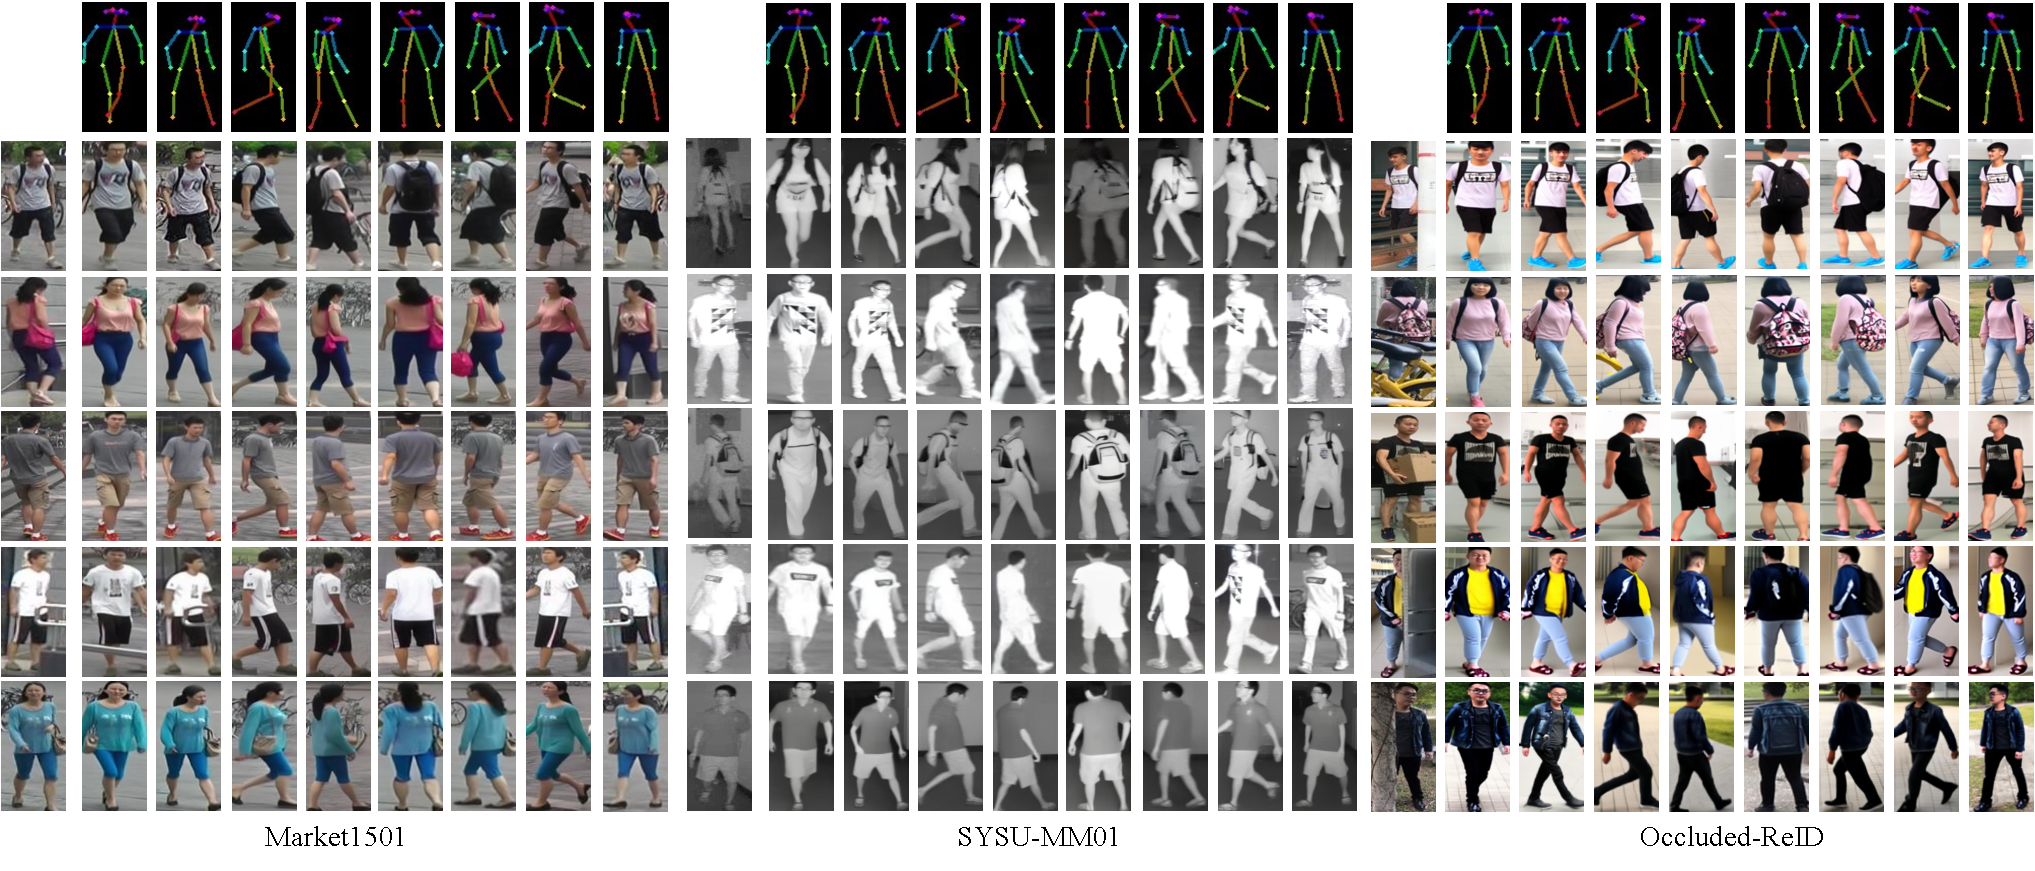
\includegraphics[width=0.8\textwidth]{figs/pdf/visualization.pdf} 
    \captionof{figure}{Visualization of our Identity-Guided Pedestrian Generation model with 8 representative poses on three datasets.}
\end{center}%
}]
\renewcommand{\thefootnote}{}
\footnotetext{$\dagger$ Corresponding author. * Equal contribution.}
\footnotetext{Codes: \textit{\url{https://github.com/yuanc3/Pose2ID}}}
% \maketitle


\begin{abstract}
Fine-tuning provides an effective means to specialize pre-trained models for various downstream tasks. However, fine-tuning often incurs high memory overhead, especially for large transformer-based models, such as LLMs. While existing methods may reduce certain parts of the memory required for fine-tuning, they still require caching all intermediate activations computed in the forward pass to update weights during the backward pass. In~this work, we develop \method, a method to reduce memory usage,  specifically the memory to store intermediate activations, in the fine-tuning of transformer-based models. During the backward pass, \method approximates the gradient computation by backpropagating through just a subset of input tokens. Thus, with \method, only a subset of intermediate activations are cached during the forward pass. Also, \method can be easily combined with existing methods like LoRA, further reducing the memory cost. We evaluate our approach on pre-trained transformer models with up to billions of parameters, considering the performance on multiple downstream tasks such as text classification and question answering in a few-shot learning setup. Overall, \method achieves performance on par with full fine-tuning or representative memory-efficient fine-tuning methods,  while greatly reducing the memory footprint, especially when combined with other methods with complementary memory reduction mechanisms. We hope that our approach will facilitate the fine-tuning of large transformers,  in specializing them for specific domains or co-training them with other neural components from a larger system. Our code is available at \githubURL.
\blfootnote{\textbf{*} Equal contribution}
\end{abstract}
    
\section{Introduction}
\label{sec:intro}

\begin{figure*}[t!]
    \centering
    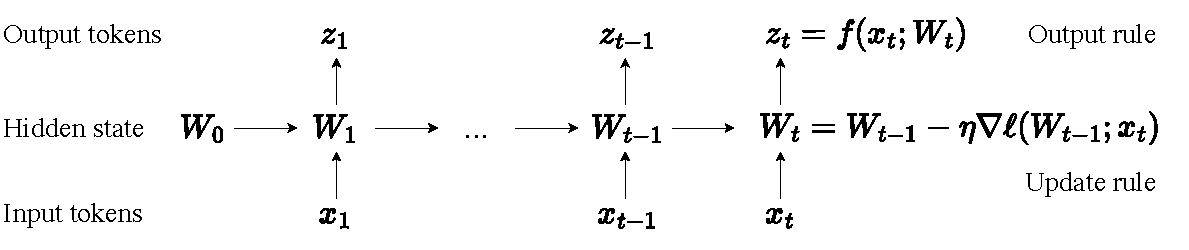
\includegraphics[width=0.8\textwidth]{figs/simple_teaser.pdf}
    \caption{All RNN layers can be expressed as a hidden state that transitions according to an update rule.
    The key idea in \cite{sun2024ttt} is to make the hidden state itself a model $f$ with weights $W$, and the update rule a gradient step on the self-supervised loss $\ell$.
    Therefore, updating the hidden state on a test sequence is equivalent to training the model $f$ at test time. 
    This process, known as Test-Time Training (TTT), is programmed into TTT layers. 
    Figure and caption taken from \cite{sun2024ttt}.
    }
    \label{fig:ttt-layer}
\end{figure*}

Despite the remarkable progress in visual and physical realism, state-of-the-art video Transformers are still generating mostly short clips of single scenes without complex stories.
At the time of writing (March 2025), the maximum length of public APIs for video generation is 20 seconds for Sora (OpenAI), 16 seconds for MovieGen (Meta), 10 for Ray~2 (Luma), and 8 for Veo~2 (Google).
None of these APIs can autonomously generate complex multi-scene stories.

A fundamental challenge behind these technical limitations is long context, because the cost of self-attention layers in Transformers increases quadratically with context length.
This challenge is especially acute for video generation with dynamic motion, whose context cannot be easily compressed by a tokenizer.
Using a standard tokenizer, each of our one-minute videos requires over 300k tokens in context. 
With self-attention, generating a one-minute video would have taken $11\times$ longer than generating 20 videos of 3 seconds each, and training would have taken $12\times$ longer.

To address this challenge, recent work on video generation has investigated RNN layers as an efficient alternative to self-attention, because their cost increases linearly with context length~\cite{wang2024lingenhighresolutionminutelengthtexttovideo}.
Modern RNN layers, especially variants of linear attention~\cite{schmidhuberlinearattn, katharopoulos2020lineartransformers} such as Mamba~\cite{gu2024mamba, dao2024mamba2} and DeltaNet~\cite{schlag2021deltanet, yang2025gateddeltanetworksimproving}, have shown impressive results for natural language tasks.
However, we have yet to see long videos with complex stories or dynamic motion generated by RNNs.
Videos (\href{https://lineargen.github.io/}{link}) in \cite{wang2024lingenhighresolutionminutelengthtexttovideo} are high resolution and one-minute long, but contain only single scenes and slow motion, let alone complex stories.

We believe that these RNN layers generate less complex videos because their hidden states are less expressive.
RNN layers can only store past tokens into a hidden state of fixed size, which is only a matrix for linear attention variants such as Mamba and DeltaNet.
It is inherently challenging to compress hundreds of thousands of vectors into a matrix with only thousands in rank.
As a consequence, these RNN layers struggle to remember the deep relationships between distant tokens.

We experiment with an alternative class of RNN layers whose hidden states themselves can be neural networks. Specifically, we use two-layer MLPs with 2$\times$ more hidden cells and richer nonlinearities than the linear (matrix) hidden states in linear attention variants.
Since the neural network hidden states are updated by training even on test sequences, these new layers are called Test-Time Training (TTT) layers~\cite{sun2024ttt}.

We start from a pre-trained Diffusion Transformer (CogVideo-X 5B \cite{hong2023cogvideo}) that could only generate 3-second short clips at 16 fps (or 6 seconds at 8 fps).
Then, we add TTT layers initialized from scratch and fine-tune this model to generate one-minute videos from text storyboards. 
We limit the self-attention layers to 3-second segments so their cost stays manageable.
With only preliminary systems optimization, our training run takes the equivalent of 50 hours on 256 H100s.

We curate a text-to-video dataset based on $\approx$ 7 hours of \textit{Tom and Jerry} cartoons with human-annotated storyboards.
We intentionally limit our scope to this specific domain for fast research iteration.
As a proof-of-concept, our dataset emphasizes complex, multi-scene, and long-range stories with dynamic motion, where progress is still needed; it has less emphasis on visual and physical realism, where remarkable progress has already been made.
We believe that improvements in long-context capabilities for this specific domain will transfer to general-purpose video generation.

Compared to strong baselines such as Mamba 2~\cite{dao2024mamba2}, Gated DeltaNet~\cite{yang2025gateddeltanetworksimproving}, and sliding-window attention layers, TTT layers generate much more coherent videos that tell complex stories with dynamic motion, leading by 34 Elo points in a human evaluation of 100 videos per method.
For context, GPT-4o scores 29 Elo points over GPT-4 Turbo in LMSys Chatbot Arena~\cite{chiang2024chatbot}.

Sample videos, code and annotations are available at:
\url{https://test-time-training.github.io/video-dit}
\section{Related works}
\paragraph{Person Re-Identification}
Person re-identification (ReID) is a critical task in computer vision that focuses on identifying individuals across different camera views. It plays a significant role in surveillance and security applications. Recent advancements in ReID have leveraged deep learning techniques to enhance performance, particularly using convolutional neural networks (CNNs\cite{krizhevsky2012imagenet}) and vision transformers (ViTs \cite{alexey2020image}). The deep learning based methods\cite{bak2010person, layne2012person, sun2017svdnet, hermans2017defense, liao2020interpretable, fu2021unsupervised, zhang2023protohpe, zhang2023pha} that focus on feature extraction and metric learning\cite{koestinger2012large, hirzer2012relaxed, liao2015efficient, yu2018unsupervised} have improved feature extraction by learning robust and discriminative embeddings that capture identity-specific information.

Standard datasets like Market-1501 \cite{zheng2015scalable} have been widely used to benchmark ReID algorithms under normal conditions. Moreover, there are some challenging scenarios such as occlusions and cross-modality matching. Occluded-REID \cite{zhuo2018occluded} addresses the difficulties of identifying partially obscured individuals, while SYSU-MM01 \cite{wu2017rgb} focuses on matching identities between visible and infrared images, crucial for nighttime surveillance.

\paragraph{Feature Enhancement in Re-Identification}
Extracting robust feature representations is one of the key challenges in re-identification. Feature enhancement could help the ReID model easily differentiate between two people. Data augmentation techniques\cite{mclaughlin2015data, zhong2020random, ma2019true} were enhanced for feature enhancement. By increasing the diversity of training data, ReID model could extract robust and discriminative features.

Apart from improving the quality of the generated images, some Gan-based methods couple feature extraction and data generation end-to-end to distill identity related feature. FD-GAN\cite{ge2018fd} separates identity from the pose by generating images across multiple poses, enhancing the ReID system's robustness to pose changes. Zheng et al.\cite{zheng2019joint} separately encodes each person into an appearance code and a structure code. Eom el al.\cite{eom2019learning} propose to disentangle identity-related and identity-unrelated features from person images.  However, GAN-based methods face challenges such as training instability and mode collapse, which may not keep identity consistency.

In addition, the re-ranking technique refines feature-based distances to improve ReID accuracy. Such as k-Reciprocal Encoding Re-ranking\cite{zhong2017re}, which improves retrieval accuracy by leveraging the mutual neighbors between images to refine the distance metric. 

\paragraph{Person Generation Models}
Recent approaches have incorporated generative models, particularly generative adversarial networks (GANs) \cite{goodfellow2014generative}, to augment ReID data or enhance feature quality. Style transfer GAN-based methods\cite{zhong2018camstyle, dai2018cross, huang2019sbsgan, pang2022cross} transfer labeled training images to artificially generated images in diffrent camera domains, background domains or RGB-infrared domains. Pose-transfer GAN-based methods\cite{siarohin2018deformable,qian2018pose, liu2018pose, borgia2019gan, zhang2020pac} enable the synthesis of person images with variations in pose and appearance, enriching the dataset and making feature representations more robust to changes in poses. Random generation GAN-based mothods \cite{zheng2017unlabeled, ainam2019sparse, hussin2021stylegan} generate random images of persons and use Label Smooth Regularization (LSR \cite{szegedy2016rethinking}) or other methods to automatically label them. However, these methods often struggle to maintain identity consistency in pose variation, as generated images are susceptible to identity drift. 
The emergence of diffusion models has advanced the field of generative modeling, showing remarkable results in image generation tasks \cite{ho2020denoising}. Leveraging the capabilities of pre-trained models like Stable Diffusion \cite{rombach2022high}, researchers have developed techniques\cite{bhunia2023person, zhang2023adding} to generate high-quality human images conditioned on 2D human poses. Such as ControlNet\cite{zhang2023adding}, which integrates conditional control into diffusion models, allowing precise manipulation of generated images based on pose inputs.


% TO BE DONE


% In our work, we propose a framework that utilizes the inherent generalizability of existing diffusion models to generate different poses of the same individual based on reference images and target pose information. By extracting features from these generated images, we aim to enhance the original features without any extra parameters. This approach focuses on improving feature quality during inference and can be seamlessly integrated into various ReID tasks, including standard, occluded, and cross-modality scenarios. It can be used with various SOTA ReID model.
\section{Vision as LoRA}
\label{sec:methods}
\begin{figure*}
    \centering
    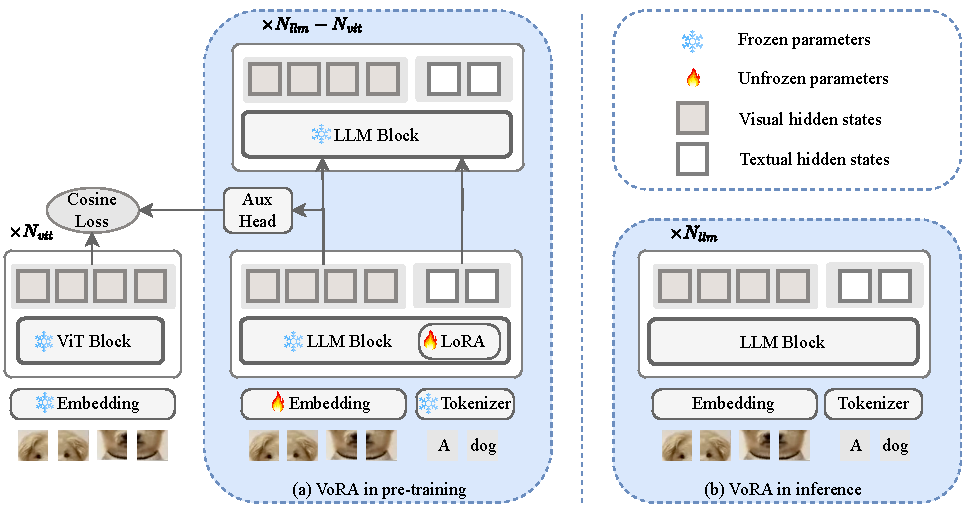
\includegraphics[width=\linewidth]{images/Figure2.pdf}
    \caption{The architecture of \model{}. Figure (a) shows the architecture of \model{} in pre-training: in this stage, \model{} only unfreezes the LoRA layers for vision and the visual embedding layer, i.e., a shallow MLP layer with a positional embedding. Figure (b) shows \model{} in inference: the LoRA layers are merged into the LLM, and thus the only added parameters are a shallow embedding layer (about 6M parameters).}
    \label{fig:architecture}
\end{figure*}
In this section, we introduce three key components of \model{}: vision as LoRA, block-wise distillation, and bi-directional attention masks for vision. 

\subsection{Stabilize training: Vision as LoRA}

As shown in Figure \ref{fig:architecture}(a), we integrate LoRA layers into the LLM to enable vision understanding. During pre-training, images are first converted into vision embeddings using a lightweight embedding layer, i.e., a shallow MLP with positional encodings of about 6M parameters. Let $N_{\text{vit}}$ and $N_{\text{llm}}$ denote the number of blocks in the ViT and the LLM, respectively. We apply LoRA to all linear layers within the first $N_{\text{vit}}$ blocks of the LLM, including query-key-value (QKV) projections and feed-forward network (FFN) layers. Crucially, only the LoRA parameters and the vision embedding layer are updated during training, while the original LLM parameters remain frozen. This design decouples vision and language parameters, stabilizing training compared to full LLM training and avoiding the training collapse observed in prior works \cite{eve}.

Figure \ref{fig:architecture}(b) demonstrates that after pre-training, the LoRA parameters can be seamlessly merged into the base LLM, thereby eliminating additional inference overhead. 

% \subsection{Boost training: Block-wise distillation}
% \label{sec:distillation}

% Our framework introduces a block-wise distillation paradigm that aligns \model{}'s emerging visual representations with the hierarchical feature spaces of a pre-trained Vision Transformer (ViT). This strategic alignment harnesses the ViT's rich visual priors to accelerate training while mitigating dependence on large-scale multimodal datasets.  


% Our core idea is to align \model{}’s visual representations with those of a pre-trained ViT, leveraging the ViT’s strong visual priors to boost training and reduce reliance on large-scale training data. To achieve this, we adopt knowledge distillation \cite{distillation}, transferring visual knowledge from the ViT into \model{}. Unlike traditional distillation methods that train an entire model, our approach updates only the LoRA layers for vision within the LLM. This ensures that the LoRA layers directly learn visual knowledge from the ViT while maintaining the LLM’s original capabilities. Specifically, for block $i$ among the first $N_{vit}$ blocks in LLM, we align its output hidden states with those of block $i$ in the ViT.
% Additionally, we require \model{} to predict a caption given an image, providing additional supervision. 
% The training objective consists of the following three components.

% \textbf{Distillation Loss.} For each transformer block $i$ and visual embedding position $s$, we compute cosine similarity between projected LLM features and ViT embeddings:
% \begin{equation}
%     \mathcal{L}_{\text{distill}}^i = \frac{1}{S} \sum_{s=1}^S \left( 1 - \frac{
%         \mathrm{AuxHead}(\bm{h}_{\text{LLM}}^{i,s})^\top \bm{h}_{\text{ViT}}^{i,s}
%     }{
%         \|\mathrm{AuxHead}(\bm{h}_{\text{LLM}}^{i,s})\|_2 \|\bm{h}_{\text{ViT}}^{i,s}\|_2
%     } \right),
% \end{equation}
% where $S$ is visual sequence length, i.e. the vision token count of the ViT, $\bm{h}_{\text{LLM}}^{i,s}, \bm{h}_{\text{ViT}}^{i,s} \in \mathbb{R}^M$ are visual hidden states for the $s$-th token in block $i$, and $\mathrm{AuxHead}(\cdot)$ is a shallow head consisting of an RMSNorm layer and a linear layer. The distillation loss is averaged across $N_{\text{ViT}}$ blocks:
% \begin{equation}
%     \mathcal{L}_{\text{distill}} = \frac{1}{N_{\text{ViT}}} \sum_{i=1}^{N_{\text{ViT}}} \mathcal{L}_{\text{distill}}^i.
% \end{equation}

% \textbf{Language Modeling Loss.} For each image-caption pair, we compute cross-entropy only on caption starting from position $t_0$:
% \begin{equation} 
%     \mathcal{L}_{\text{LM}} = -\sum_{t=t_0}^T \log P(w_t | w_{<t}, \bm{x}_{\text{image}}),
% \end{equation}
% where $T$ is the total sequence length and $\bm{x}_{\text{image}}$ denotes visual inputs.

% \textbf{Total Objective.} The final loss combines both distillation loss and language modeling loss:
% \begin{equation}
%     \mathcal{L}_{\text{total}} = \mathcal{L}_{\text{distill}} + \mathcal{L}_{\text{LM}}.
% \end{equation}
\subsection{Boost training: block-wise distillation}
\label{sec:distillation}

We introduce a block-wise distillation paradigm to align \model{}'s intermediate visual representations with the block-wise features of a pre-trained ViT. This approach transfers visual knowledge from the ViT via knowledge distillation \cite{distillation, eva}, accelerating training while reducing dependence on large-scale vision data. Unlike conventional distillation that updates entire models, we only update the vision-specific LoRA layers within the LLM. Specifically, for each block $i$ in the first $N_{\text{vit}}$ layers of the LLM, we align its hidden states with those of block $i$ in the ViT. 
The training objective combines the following two components.
\\
\textbf{Distillation loss.} For each transformer block $i$ and vision token position $s$, we maximize cosine similarity between projected LLM features and ViT embeddings via:
\begin{equation}
    \mathcal{L}_{\text{distill}}^i = \frac{1}{S} \sum_{s=1}^S \left( 1 - \frac{
        \mathrm{AuxHead}(\bm{h}_{\text{llm}}^{i,s})^\top \bm{h}_{\text{vit}}^{i,s}
    }{
        \|\mathrm{AuxHead}(\bm{h}_{\text{llm}}^{i,s})\|_2 \|\bm{h}_{\text{vit}}^{i,s}\|_2
    } \right),
\end{equation}
where $S$ is the ViT's output sequence length (number of vision embeddings to represent one image), $\bm{h}_{\text{llm}}^{i,s}, \bm{h}_{\text{vit}}^{i,s} \in \mathbb{R}^M$ denote the hidden states for the $s$-th token in block $i$, and $\mathrm{AuxHead}(\cdot)$ is a projection layer (RMSNorm \cite{rmsnorm} + linear layer) adapting LLM features to the ViT's embedding space. The loss is averaged across $N_{\text{vit}}$ blocks:
\begin{equation}
    \mathcal{L}_{\text{distill}} = \frac{1}{N_{\text{vit}}} \sum_{i=1}^{N_{\text{vit}}} \mathcal{L}_{\text{distill}}^i.
\end{equation}
\\
\textbf{Language modeling loss.} For image-caption pairs, we optimize caption generation using cross-entropy, which is consistent with the standard approach used in LLMs:
\begin{equation} 
    \mathcal{L}_{\text{LM}} = -\sum_{t=t_0}^T \log P(w_t | w_{<t}, \bm{x}_{\text{image}}),
\end{equation}
where $T$ is the total sequence length, $\bm{x}_{\text{image}}$ represents vision inputs, and $t_0$ indexes the first caption token.
\\
\textbf{Final objective.} The final loss combines both objectives:
\begin{equation}
    \mathcal{L}_{\text{total}} = \mathcal{L}_{\text{distill}} + \mathcal{L}_{\text{LM}}.
\end{equation}

\subsection{Bi-directional attention masks for vision}

\begin{figure}
    \centering
    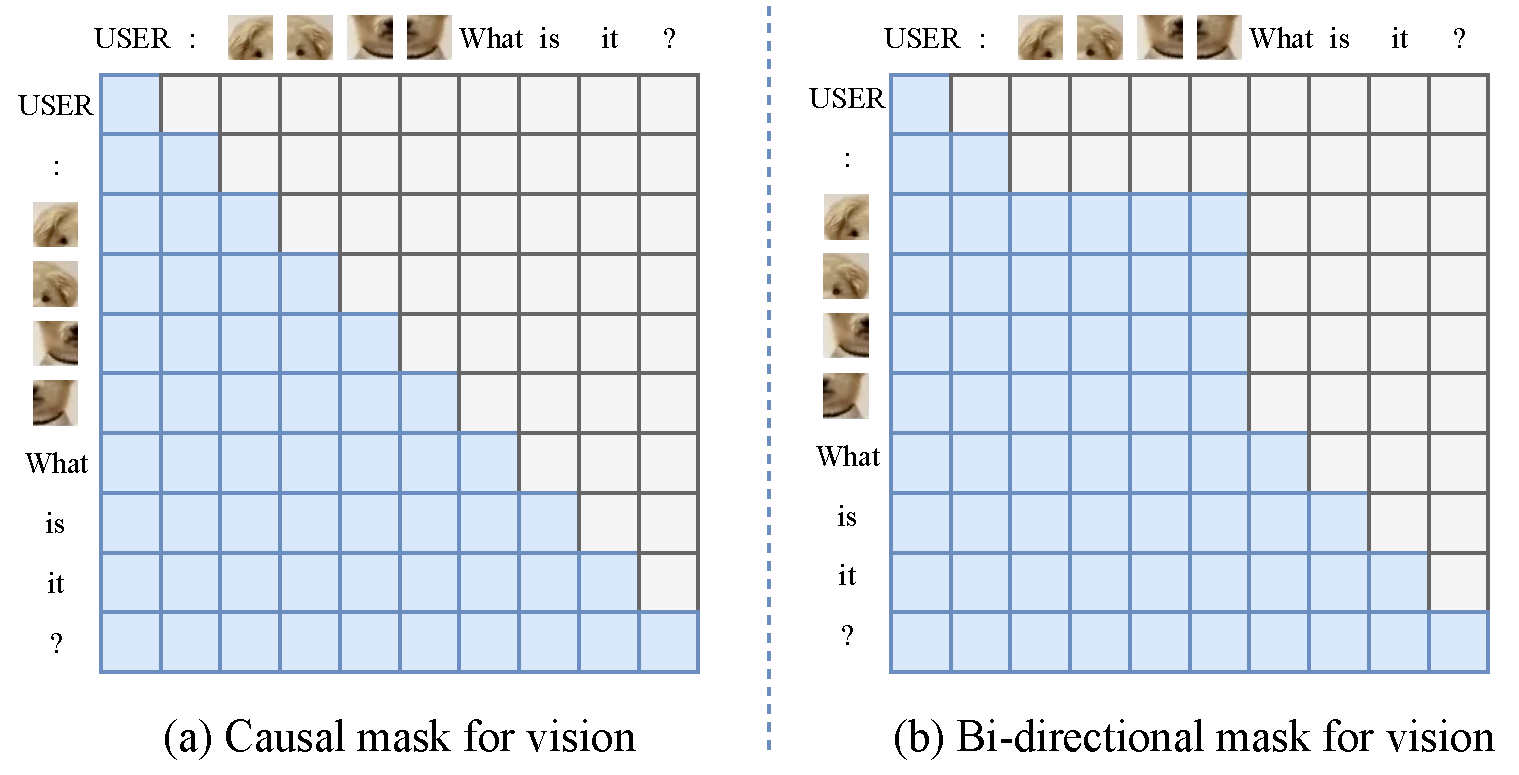
\includegraphics[width=\linewidth]{images/Figure3.pdf}
    \caption{Attention masks for vision: (a) causal attention inherits the autoregressive mask from language modeling, enforcing sequential dependency between image patches; (b) bidirectional attention offers full visibility between all image patches within the same input, enabling global contextual awareness.}
    \label{fig:attention-mask}
\end{figure}

While bi-directional attention masks is common in Transformer architectures in various fields \cite{vit, clip, transfusion}, few studies have explored replacing the causal mask of autoregressive LLMs with a bi-directional mask, especially in the field of MLLMs.

As illustrated in Figure \ref{fig:attention-mask}, we have explored the use of a bi-directional attention mask for vision. Our findings indicate that this attention mask positively impacts the final performance of \model{}, which will be discussed in Section \ref{sec:experiments}. In contrast to prior works \cite{eve, evev2, monointernvl, fuyu}, which have relied on causal masking designed for autoregressive text generation, we demonstrate that adopting bi-directional attention for vision tokens while retaining causal masking for text, not only preserves language capabilities but also enhances visual performance. This aligns with insights from image generation research \cite{transfusion}, highlighting \model{}’s potential as a unified architecture for multimodal generation and understanding tasks.
% \\
% As shown in Figure \ref{fig:attention-mask}, we explored three types of attention masks for vision: (a) causal mask, (b) bidirectional mask, and (c) localized bidirectional mask. While the bidirectional mask demonstrates improved performance, we find that the localized bidirectional mask outperforms it by allowing tokens to focus exclusively on a single image without interference from other text.
% \subsection{Simple Image Patchifier}

% Since we employ \model{} to encode visual information, we can utilize a very lightweight image patchifier. For simplicity, we use the original image patchifier from ViT, along with a single linear layer to align the dimensions, resulting in less than 10M parameters.





\begin{table*}[ht]
\centering
\small
\renewcommand{\arraystretch}{0.95}
\renewcommand\tabcolsep{4pt}
\begin{tabular}{cc|c|c|c|c|ccc}
\hline 
\multicolumn{2}{c|}{Dataset} & Model & Venue & Base & Method & mAP$\uparrow$ & Rank-1$\uparrow$ & $\text{ID}^2$$\downarrow$ \\ \hline
% \multicolumn{2}{c|}{} & & & & ori & 3.34 & 11.4 & 0.5135 \\ \cline{6-9} 
% \multicolumn{2}{c|}{} & \multirow{-2}{*}{TransReID\cite{he2021transreid}(w/o training)} & & & +ours & 52.81\scriptsize{(+49.47)} & 78.92\scriptsize{(+67.52)} & 0.2158 \\ \cline{3-3} \cline{6-9} 
\multicolumn{2}{c|}{} & & & & official & 79.88 & 91.48 & 0.2193 \\ \cline{6-9} 
\multicolumn{2}{c|}{} & \multirow{-2}{*}{TransReID\cite{he2021transreid}(w/o camid)} & & & +ours & 90.39\scriptsize{(+10.51)} & 94.74\scriptsize{(+3.26)} & 0.1357 \\ \cline{3-3} \cline{6-9} 
\multicolumn{2}{c|}{} & & & & official & 89 & 95.1 & 0.2759 \\ \cline{6-9} 
\multicolumn{2}{c|}{} & \multirow{-2}{*}{TransReID\cite{he2021transreid}(w/ camid)} & \multirow{-4}{*}{ICCV21} & \multirow{-4}{*}{ViT} & +ours & 93.01\scriptsize{(+4.01)} & 95.52\scriptsize{(+0.42)} & 0.1967 \\ \cline{3-9} 
\multicolumn{2}{c|}{} & & & & official & 89.7 & 95.4 & 0.0993 \\ \cline{6-9} 
\multicolumn{2}{c|}{} & & & \multirow{-2}{*}{ViT} & +ours & 94\scriptsize{(+4.3)} & 96.4\scriptsize{(+1.0)} & 0.0624 \\ \cline{5-9} 
\multicolumn{2}{c|}{} & & & & official & 89.8 & 95.7 & 0.0877 \\ \cline{6-9} 
\multicolumn{2}{c|}{\multirow{-8}{*}{Market1501}} & \multirow{-4}{*}{CLIP-ReID\cite{li2023clip}} & \multirow{-4}{*}{AAAI23} & \multirow{-2}{*}{CNN} & \cellcolor{gray!20}+ours & \cellcolor{gray!20}94.9\scriptsize{(+5.1)} & \cellcolor{gray!20}97.3\scriptsize{(+1.6)} & \cellcolor{gray!20}0.053 \\ \hline
\multicolumn{2}{c|}{} & & & & official & 79.05 & 85.4 & 0.3124 \\ \cline{6-9} 
\multicolumn{2}{c|}{} & \multirow{-2}{*}{KPR\cite{somers2025keypoint}} & \multirow{-2}{*}{ECCV24} & \multirow{-2}{*}{ViT} & \cellcolor{gray!20}+ours & \cellcolor{gray!20}89.34\scriptsize{(+10.29)} & \cellcolor{gray!20}91\scriptsize{(+5.6)} & \cellcolor{gray!20}0.1434 \\ \cline{3-9} 
\multicolumn{2}{c|}{} & & & & official & 70.41 & 77.2 & 0.377 \\ \cline{6-9} 
\multicolumn{2}{c|}{\multirow{-4}{*}{Occluded-ReID}} & \multirow{-2}{*}{BPBReID\cite{somers2023body}} & \multirow{-2}{*}{WACV23} & \multirow{-2}{*}{ViT} & +ours & 86.05\scriptsize{(+15.64)} & 89.1\scriptsize{(+11.9)} & 0.1504 \\ \hline
\multicolumn{1}{c|}{} & & & & & official & 71.81 & 75.29 & 0.4817 \\ \cline{6-9} 
\multicolumn{1}{c|}{} & \multirow{-2}{*}{All} & & & & \cellcolor{gray!20}+ours & \cellcolor{gray!20}76.44\scriptsize{(+4.63)} & \cellcolor{gray!20}79.33\scriptsize{(+4.04)} & \cellcolor{gray!20}0.4072 \\ \cline{2-2} \cline{6-9} 
\multicolumn{1}{c|}{} & & & & & official & 84.6 & 81.59 & 0.4424 \\ \cline{6-9} 
\multicolumn{1}{c|}{} & \multirow{-2}{*}{Indoor} & \multirow{-4}{*}{SAAI\cite{fang2023visible}} & \multirow{-4}{*}{ICCV23} & \multirow{-4}{*}{CNN} & \cellcolor{gray!20}+ours & \cellcolor{gray!20}86.83\scriptsize{(+2.23)} & \cellcolor{gray!20}84.2\scriptsize{(+2.61)} & \cellcolor{gray!20}0.3694 \\ \cline{2-9} 
\multicolumn{1}{c|}{} & & & & & official & 66.13 & 67.7 & 0.4308 \\ \cline{6-9} 
\multicolumn{1}{c|}{} & \multirow{-2}{*}{All} & & & & +ours & 75.43\scriptsize{(+9.3)} & 74.81\scriptsize{(+7.11)} & 0.3133 \\ \cline{2-2} \cline{6-9} 
\multicolumn{1}{c|}{} & & & & & official & 77.81 & 72.95 & 0.4046 \\ \cline{6-9} 
\multicolumn{1}{c|}{\multirow{-8}{*}{SYSU-MM01}} & \multirow{-2}{*}{Indoor} & \multirow{-4}{*}{PMT\cite{lu2023learning}} & \multirow{-4}{*}{AAAI23} & \multirow{-4}{*}{ViT} & +ours & 84.29\scriptsize{(+6.48)} & 80.29\scriptsize{(+7.34)} & 0.2995 \\ \hline
\end{tabular}

\caption{Improvements with our method on different SOTA models with both ViT and CNN backbone on Market1501, SYSU-MM01, and Occluded-ReID datasets. The data under \colorbox{gray!20}{grey} is the new SOTA with our methods of that dataset.}
\label{tab:sota}
\end{table*}


\begin{table*}[ht]
\centering
\small
\renewcommand{\arraystretch}{1.0}
\renewcommand\tabcolsep{4pt}
\begin{minipage}{0.32\textwidth}
\centering
\begin{tabular}{c|ccc}
\hline
\textbf{Methods} & mAP$\uparrow$ & Rank-1$\uparrow$ & $\text{ID}^2$$\downarrow$ \\ \hline
Base & 79.88 & 91.48 & 0.2193 \\
+NFC & 83.92 & 91.83 & 0.1824 \\
+IPG & 88.02 & 94.77 & 0.1553 \\
\rowcolor{gray!20}
+NFC+IPG & 90.39 & 94.74 & 0.1357 \\
\hline
\end{tabular}
\caption{Ablation study on effects of feature centralization through Identity-Guided Pedestrian Generation (IPG) and Neighbor Feature Centralization (NFC).}
\label{tab:ablation_fe_pg}
\end{minipage}
\hfill
\begin{minipage}{0.32\textwidth}
\centering
\begin{tabular}{cc|cc}
\hline
$\text{Gallery}^\text{NFC}$ & $\text{Query}^\text{NFC}$  & mAP$\uparrow$ & Rank-1$\uparrow$ \\ \hline
 \ding{55} & \ding{55}   & 79.88&	91.48  \\
 \ding{51} & \ding{55}    & 81.70 & 92.04  \\
\ding{55} & \ding{51}    & 82.76 & 91.69  \\
\rowcolor{gray!20}
\ding{51} & \ding{51}    & 83.92 & 91.83 \\ 
\hline
\end{tabular}
\caption{Ablation study of Neighbor Feature Centralization (NFC) Algorithm on Market1501 dataset. We test on the gallery and query set respectively.}
\label{tab:as_fe}
\end{minipage}
\hfill
\begin{minipage}{0.32\textwidth}
\centering
\begin{tabular}{cc|cc}
\hline
% \multicolumn{2}{c|}{\textbf{Methods}}& \multicolumn{4}{c}{Metrics}  \\ \hline
$\text{Gallery}^\text{IPG}$ & $\text{Query}^\text{IPG}$  & mAP$\uparrow$ & Rank-1$\uparrow$ \\ \hline
\ding{55} & \ding{55}   & 79.88&	91.48  \\
% \ding{51} & \ding{55}    &  84.06 &91.48 \\
% \ding{55} & \ding{51}    & 81.01 &91.03  \\
% \rowcolor{gray!20}
% \ding{51} & \ding{51}    & 87.38& 94.63 \\ 
 \ding{51} & \ding{55}    & 84.65&	92.07  \\
\ding{55} & \ding{51}    & 82.18	&92.40  \\
\rowcolor{gray!20}
\ding{51} & \ding{51}    &88.02&	94.77 \\ 
\hline
\end{tabular}
\caption{Ablation study of Feature ID-Centralizing with Pedestrian Generation (IPG) on Market1501. We test on gallery and query set respectively.}
\label{tab:as_gen}
\end{minipage}
\end{table*}


\begin{table}
\small
    \centering
    \renewcommand{\arraystretch}{1}
    \renewcommand\tabcolsep{6pt}
    \begin{tabular}{c|ccccc}
        \hline
        \textbf{Method} & mAP$\uparrow$ & R1$\uparrow$ & R5$\uparrow$ & R10$\uparrow$ & $\text{ID}^2$$\downarrow$ \\ \hline
        w/o training & 3.34 & 11.4 & 21.88 & 28 & 0.5135 \\
        \rowcolor{gray!20}
        +IPG & 52.81 & 78.92 & 91.21 & 94.27 & 0.2158 \\
        \rowcolor{gray!20}
        +IPG+NFC & 57.27 & 82.39 & 90.17 & 92.81 & 0.1890 \\ \hline
    \end{tabular}
    \caption{ReID performance on Market1501 with only ImageNet pre-trained weights without ReID training. The distribution visualized in Fig.\ref{fig:noise_tsne}.}
    \label{tab:notraining}
\end{table}
\begin{figure}[H]
\centering
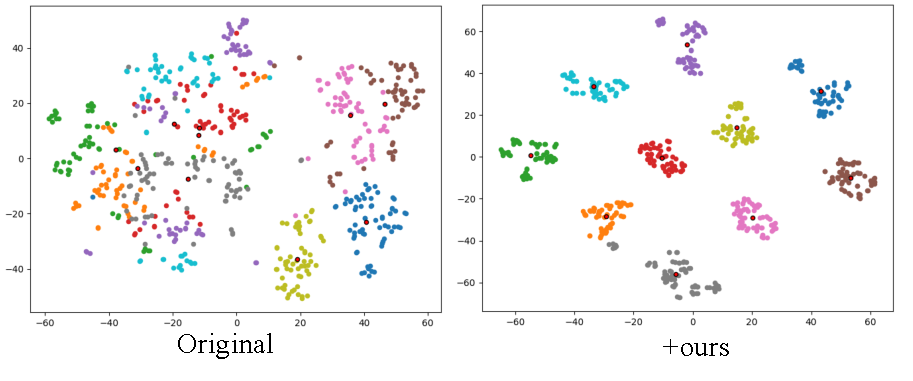
\includegraphics[width=0.95\linewidth]{figs/pdf/noise_tsne.pdf}
\caption{t-SNE visualization of 10 IDs feature distribution with and without our method on ImageNet pre-trained weights.}
\label{fig:noise_tsne}
\end{figure}


\section{Experiments}
\subsection{Implementation Details}

\textbf{Data Cleaning.}
Training an effective generative model requires high-quality data support. In current ReID (Person Re-Identification) datasets, there are many low-quality images, and removing them can help reduce interference to the model. In our experiments, we found two main issues that need to be addressed:\textbf{Extremely Low-quality Images}: The dataset contains images with such low resolution that even the human eye cannot recognize them as a "person". \textbf{Pose Estimation Failures}: The pose estimation model inevitably fails to detect pedestrian poses in some images.

Utilizing the feature distribution mentioned in Section\ref{Feature Distribution}, we can solve the issues and get the reference image set $S_i^{\text{ref}}$ and target image set $S^{\text{trg}}_i$ of identity $i$.
The cleansing process is detailed in \textbf{Supplementary}. 
\\
\textbf{Identity-guided Pedestrian Generation model details}
For the reference UNet and denoising UNet, we use the pretrained weights of Stable Diffusion v1.5\cite{rombach2022high}. The VAE encoder and decoder initialized with official weights\cite{kingma2013auto} and froze. For the ReID model, we use pre-trained TransReID\cite{he2021transreid} without cameras on Market1501 and freeze. 

The training data collected from training set of Market1501\cite{zheng2015scalable},  Mars\cite{zheng2016mars}, MSMT17\cite{wei2018person} and SYSU-MM01\cite{wu2017rgb}, with a total of 1946 different IDs. The model was trained for 80,000 iterations on one L20(48G) GPU with batch size of 4, which costs about 20 hours, and optimized by Adam\cite{kingma2014adam} with a learning rate of 1e-5 and weight decay of 0.01. All images are resized to 512×256. We applied random flip and random erasing\cite{zhong2020random} data augmentation only on reference images.

According to Section\ref{standard pose}, we selected 8 poses on the market1501 dataset as the representative poses. Each image in test set generates 8 images with these representative poses. The generation uses DDIM with 20 steps, classifier-free guidance with a scale of 3.5, and generator seed of 42.
\\
\textbf{ReID test settings}
Test models are loaded with official open-source pre-trained models for testing. In addition, considering the generated images do not have camera IDs, so for feature consistency, we test without camera IDs (e.g. TransReID). To validate the effectiveness of our proposed method, image flip (Section\ref{flip}) trick is \textbf{NOT} applied in our experiments. On Market1501, set \(\eta=2\), and \(k_1=k_2=2\). On Occluded REID, set \(\eta=1\), and \(k_1=k_2=1\). On SYSU-MM01, set \(\eta=1/4\), and \(k_1=k_2=2\). The parameters analysis detailed in \textbf{Supplementary}.



\subsection{Improvements on State-of-the-art Methods}
To verify the exceptional feature enhancement performance of our framework, we selected state-of-the-art models of three ReID tasks, divided into CNN and ViT-based models, to demonstrate that our theory can apply to any model and various ReID tasks. As shown in Table.\ref{tab:sota}, we achieved excellent enhancements on different models.

It is worth mentioning that we help models achieve new \textbf{SOTAs} without re-rank on 3 benchmarks:
\begin{itemize}
    \item[$\bullet$] \textbf{CNN-base CLIP-ReID on market1501: }
    
    \setlength{\parindent}{1em} mAP 94.9\%, Rank-1 97.3\%. 
    \item[$\bullet$] \textbf{KPR on Occluded-ReID: }

    \setlength{\parindent}{1em} mAP 89.34\%, Rank-1 91\%
    
    \item[$\bullet$] \textbf{SAAI on SYSU-MM01: }

    \setlength{\parindent}{1em} All-search mode: mAP 76.44\%, Rank-1 79.33\%
    
    \setlength{\parindent}{1em} Indoor-search mode: mAP 86.83\%, Rank-1 84.2\%
\end{itemize}



\subsection{ReID without Training}
TransReID loads a ViT pre-trained model on ImageNet for training on the ReID task. The pre-training method is based on contrastive learning strategies. According to the description in Section\ref{Feature Distribution}, training with contrastive loss helps to cluster features of same label samples. Images generated by our Pedestrian Generation model exhibit identity consistency, meaning they possess the attributes of the same label. Therefore, even if the features of an individual sample lack the pedestrian matching capability, as shown in the first row of Tab.\ref{tab:notraining}, its mAP and Rank-1 are only 3.34\% and 11.4\%. However, with our method, it improved 53.93\%/70.99\% to 57.27\%/82.39\%. Additionally, we visualized of 10 IDs' feature distributions using t-SNE as shown in Fig.\ref{fig:noise_tsne}.


\begin{figure}
\centering
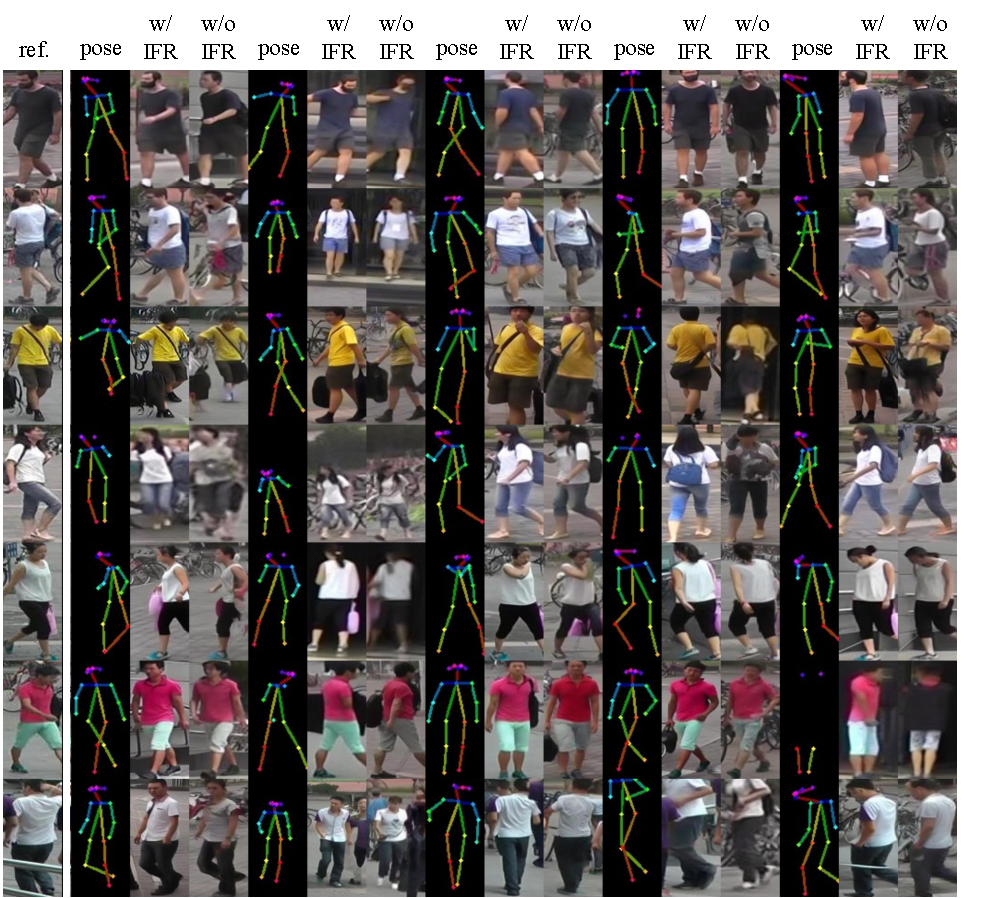
\includegraphics[width=0.95\linewidth]{figs/pdf/IFR.pdf}
\caption{The effects with and without the IFR module were visualized with five different poses randomly selected for each reference picture.}
\label{fig:IFR}
\end{figure}

\begin{table}
\small
    \centering
    \renewcommand{\arraystretch}{1}
    \renewcommand\tabcolsep{2pt}
    \begin{tabular}{c|ccc|ccc|ccc}
        \hline
        \multirow{2}{*}{\textbf{N}} & \multicolumn{3}{c|}{$\text{Gallery}^\text{IPG}$} & \multicolumn{3}{c|}{$\text{Query}^\text{IPG}$} & \multicolumn{3}{c}{$\text{Gallery}^\text{IPG}$+$\text{Query}^\text{IPG}$} \\ \cline{2-10}
          & mAP$\uparrow$ & R1$\uparrow$ & $\text{ID}^2$$\downarrow$ & mAP$\uparrow$ & R1$\uparrow$ & $\text{ID}^2$$\downarrow$ & mAP$\uparrow$ & R1$\uparrow$ & $\text{ID}^2$$\downarrow$ \\ \hline
        0 & 79.88 & 91.48 & 0.2313 & 79.88 & 91.48 & 0.1623 & 79.88 & 91.48 & 0.2193 \\
        1 & 80.96 & 90.97 & 0.2087 & 79.99 & 90.83 & 0.1363 & 82.13 & 92.01 & 0.1961 \\
        2 & 82.86 & 91.45 & 0.1904 & 81.17 & 92.04 & 0.1156 & 85.27 & 93.71 & 0.1773 \\
        3 & 83.42 & 91.75 & 0.1837 & 81.55 & 92.25 & 0.1077 & 86.16 & 94.21 & 0.1704 \\
        4 & 83.81 & 92.1  & 0.1795 & 81.76 & 92.34 & 0.1027 & 86.75 & 94.24 & 0.1661 \\
        5 & 84.07 & 91.83 & 0.1758 & 81.85 & 92.07 & 0.0984 & 87.23 & 94.71 & 0.1623 \\
        6 & 84.3  & 91.98 & 0.1730 & 81.96 & 92.52 & 0.0950 & 87.52 & 94.63 & 0.1593 \\
        7 & 84.49 & 91.86 & 0.1707 & 82.03 & 92.37 & 0.0922 & 87.76 & 94.60 & 0.1570 \\
        \rowcolor{gray!30}
        8 & 84.65 & 92.07 & 0.1691 & 82.18 & 92.40 & 0.0902 & 88.02 & 94.77 & 0.1553 \\ \hline
    \end{tabular}
    \caption{Performance Comparison by adding numbers of generated images for each image on gallery, query, and both}
    \label{tab:num}
\end{table}

\subsection{Abilation Study}
\textbf{Impact of the NFC and IPG.}
We conducted comprehensive ablation experiments on Neighbor Feature Centralization (NFC) and Feature ID-Centralizing through Identity-Guided Generation (IPG) methods. As shown in Table\ref{tab:ablation_fe_pg},\ref{tab:as_fe},\ref{tab:as_gen}, which show great improvements.
\begin{figure*}
\centering
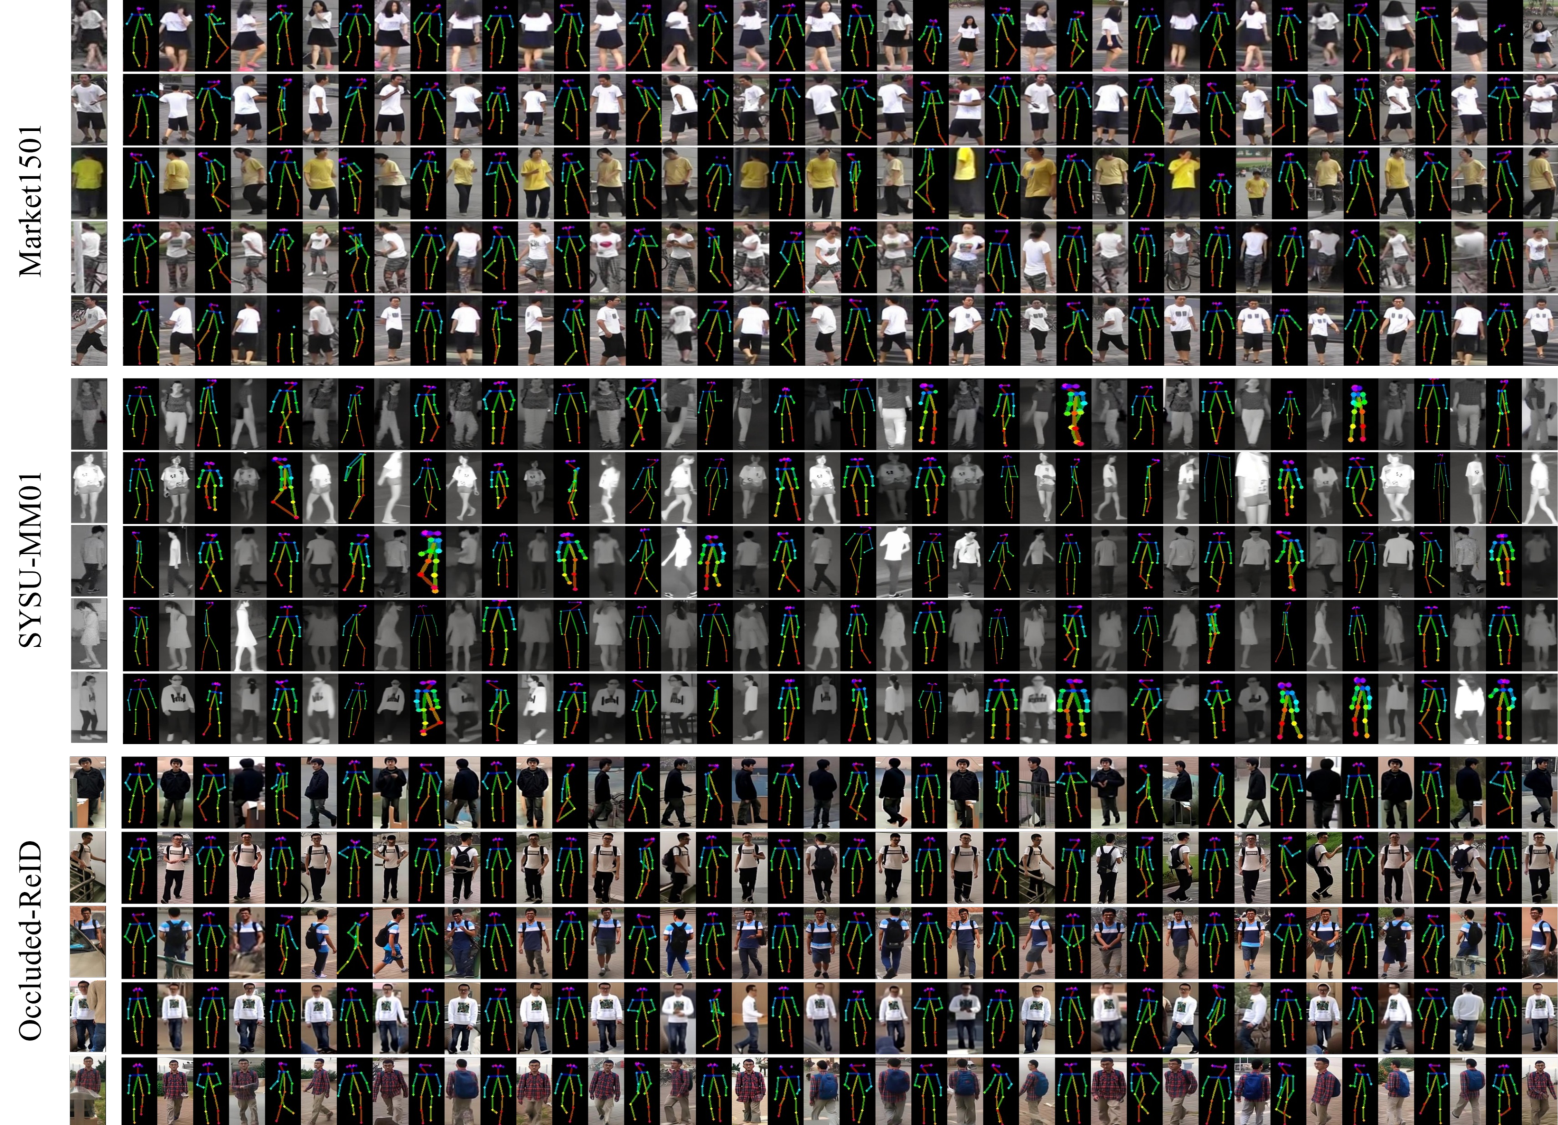
\includegraphics[width=\linewidth]{figs/pdf/random_sub_png.pdf}
\caption{Images generated with random poses. More randomly generated images can be found in Supplementary.}
\label{fig:randompose}
\end{figure*}
\\
\textbf{Effect of Feature Re-Distribute Module.}
We randomly selected 7 images from the Market1501 dataset, choosing 5 different poses for each image. We visualized the results both with and without Identity Feature Redistribute (IFR) Module. As shown in Fig.\ref{fig:IFR}, the impact of ID features on the generated outcomes is evident.
\\
\textbf{Effect of numbers of generated images.}
We randomly selected different numbers of images generated from the 8 representative poses to verify the effect of feature enhancement. As shown in Tab.\ref{tab:num}, the experimental results align with the theory mentioned in Section\ref{Feature Distribution}: the more features of the same ID that are aggregated, the more the adjustment noise extracted from individual images is reduced, enhancing the ID representation capability and resulting in improved matching performance.



\subsection{Visualizations}

\textbf{Different people with the same poses across datasets.}
We are working on Market1501, SYSU-MM01, and
Occluded-ReID datasets to visualize the 8 representative poses with only one model and results are shown in Fig.\ref{fig:intro}.
\\
\textbf{Random people with random poses.} To demonstrate the advancement of our model, as shown in Fig.\ref{fig:randompose}, we randomly chose samples from the whole dataset, and each sample randomly chose poses, including some problematic poses, fully demonstrating the diversity of model. \textbf{More examples on three datasets are visualized in }\textbf{Supplementary}.


% \subsection{Analysis on quality coefficient $\eta$ of Generation Model}

% Fig.\ref{fig:eta} illustrates the effect of adjusting the coefficient $\eta$ on the performance of the ReID model. To evaluate this impact, we gradually increased the value of $\eta$ and observed the changes in model performance on the mAP and Rank-1 metrics. 

% As the value of $\eta$ increases, the performance of the ReID model improves, reaching an optimal point. At $\eta = 2$, both mAP and Rank-1 achieve their maximum values of 88.02\% and 94.77\%, respectively. However, further increasing $\eta$ beyond this point leads to a slight decline in performance. It is easy to find that using generated images to centralize features is effective. However, considering the quality of the generated image, direct adding, although also effective, may not always achieve the best results. Therefore adjusting $\eta$ according to the generation quality of the model in this dataset can better centralize the features.
% \begin{figure}
% \centering
% 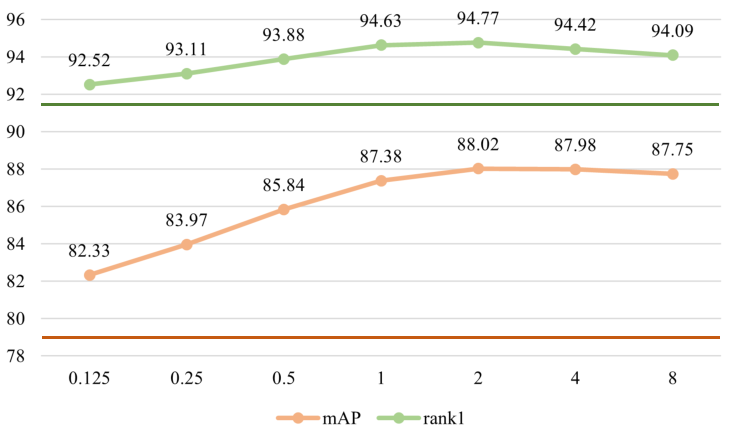
\includegraphics[width=0.9\linewidth]{figs/pdf/eta.pdf}
% \caption{Impact of the quality coefficient \( \eta \) with TransReID on Market1501. The dark color lines are the baseline.}
% \label{fig:eta}
% \end{figure}
\vspace{-5pt}
\section{Conclusion}
\vspace{-5pt}
\label{sec:conclusion}

Room reidentification is a challenging yet crucial research area, with growing applications in fields like augmented reality and homecare robotics. In this paper, we introduce AirRoom, a training-free, object-aware approach for room reidentification. AirRoom leverages multi-level object-oriented features to capture both spatial and contextual information of indoor rooms. To evaluate AirRoom, we constructed four novel datasets specifically for room reidentification. Experimental results demonstrate its robustness to viewpoint variations and superior performance over state-of-the-art methods across nearly all metrics and datasets. Furthermore, the pipeline is highly flexible, maintaining high performance without relying on specific model configurations. Collectively, our work establishes AirRoom as a powerful and versatile solution for precise room reidentification, with broad potential for real-world applications.

\begin{center}
\textbf{Acknowledgments}  
\end{center}
% This work was partially supported by the DARPA grant DARPA-PS-23-13. The views and conclusions contained in this document are those of the authors and should not be interpreted as representing the official policies, either expressed or implied, of DARPA.
\begin{sloppypar}
\noindent This work was supported by the DARPA award HR00112490426. Any opinions, findings, conclusions, or recommendations expressed in this paper are those of the authors and do not necessarily reflect the views of DARPA.
\end{sloppypar}



% \section*{Acknowledgments}
% This work was supported by the National Natural Science Foundation of China (No. 62376016).
% \clearpage
\setcounter{page}{1}
\maketitlesupplementary



\section{Methods Supplementary}
\subsection{Aggregation role of ReID loss functions}
Currently, ReID models commonly use cross-entropy loss to impose ID-level constraints, and contrastive losses (such as triplet loss) to bring features of the same ID closer while pushing apart features of different IDs. Some models also utilize center loss to construct identity centers for dynamically constraining the IDs. These methods lead to one common result: feature aggregation. From the perspective of the gradient of the loss functions, we could prove that the feature vectors of each ID in current ReID tasks naturally aggregate around a center or mean in the followings.
\paragraph{Cross-Entropy Loss} 
is often used in classification tasks, optimizing the model by maximizing the probability of the correct class. Given $N$ samples, each with a feature vector $\mathbf{z}_i \in \mathbb{R}^d$, and its corresponding class label $y_i \in \{1, 2, \dots, C\}$, the cross-entropy loss is defined as:
\begin{equation}
\mathcal{L}_{\text{CE}} = -\frac{1}{N} \sum_{i=1}^{N} \log \frac{\exp(\mathbf{w}_{y_i}^\top \mathbf{z}_i + b_{y_i})}{\sum_{j=1}^{C} \exp(\mathbf{w}_j^\top \mathbf{z}_i + b_j)}
\end{equation}
where $\mathbf{w}_j$ and $b_j$ are the weight vector and bias for class $j$, respectively.

For simplicity, assume that the final layer is a linear classifier without bias, i.e., $b_j = 0$. When the loss is minimized, the optimization objective is to maximize the score $\mathbf{w}_{y_i}^\top \mathbf{z}_i$ of the correct class while minimizing the scores $\mathbf{w}_j^\top \mathbf{z}_i$ of other classes ($j \neq y_i$).

By gradient descent optimization, we can obtain:
\begin{equation}
\frac{\partial \mathcal{L}_{\text{CE}}}{\partial \mathbf{z}_i} = 1/N\left(p_{y_i} - 1\right) \mathbf{w}_{y_i} + 1/N\sum_{j \neq y_i} p_{ij} \mathbf{w}_j
\end{equation}
where $p_{ij} = \frac{\exp(\mathbf{w}_j^\top \mathbf{z}_i)}{\sum_{k=1}^{C} \exp(\mathbf{w}_k^\top \mathbf{z}_i)}$.

With the loss function converges, $p_{y_i}\rightarrow1$ and $p_{ij}\rightarrow0 (j \neq y_i)$. The feature $\mathbf{z}_i$ is optimized to be near a linear combination of the class weight vectors $\mathbf{w}_{y_i}$. This indicates that features of the same class will tend toward a common direction, thus achieving feature aggregation.

\paragraph{Contrastive loss} (Triplet Loss as example) optimizes the feature space by bringing samples of the same class closer and pushing samples of different classes further apart. A triplet $(\mathbf{z}_a, \mathbf{z}_p, \mathbf{z}_n)$ is defined, where $\mathbf{z}_a$ is the anchor, $\mathbf{z}_p$ is the positive sample (same class), and $\mathbf{z}_n$ is the negative sample (different class). The triplet loss is defined as:
\begin{equation}
\mathcal{L}_{\text{Triplet}} = \max \left( \| \mathbf{z}_a - \mathbf{z}_p \|_2^2 - \| \mathbf{z}_a - \mathbf{z}_n \|_2^2 + \alpha, 0 \right)
\end{equation}
where $\alpha$ is the margin parameter.

To minimize the loss, the optimization objective is:
\begin{equation}
\| \mathbf{z}_a - \mathbf{z}_p \|_2^2 + \alpha < \| \mathbf{z}_a - \mathbf{z}_n \|_2^2
\end{equation}
\begin{align}
\frac{\partial \mathcal{L}_{\text{Triplet}}}{\partial \mathbf{z}_a} &= 2 (\mathbf{z}_n - \mathbf{z}_p), \\
\frac{\partial \mathcal{L}_{\text{Triplet}}}{\partial \mathbf{z}_p} &= 2 (\mathbf{z}_p - \mathbf{z}_a), \\
\frac{\partial \mathcal{L}_{\text{Triplet}}}{\partial \mathbf{z}_n} &= 2 (\mathbf{z}_a - \mathbf{z}_n).
\end{align}

By minimizing triplet loss, the feature $\mathbf{z}_p$ is pulled closer to $\mathbf{z}_a$, while $\mathbf{z}_n$ is pushed away. Through this mechanism, Triplet Loss encourages features of the same class to aggregate together while features of different classes are separated from each other.

\paragraph{Center loss} further enhances feature aggregation by introducing a feature center for each class. For each class $j$, there is a feature center $\mathbf{c}_j$, and the center loss is defined as:
\begin{equation}
\mathcal{L}_{\text{Center}} = \frac{1}{2} \sum_{i=1}^{N} \| \mathbf{z}_i - \mathbf{c}_{y_i} \|_2^2
\end{equation}

The goal of minimizing center loss is to make each sample's feature vector $\mathbf{z}_i$ as close as possible to its corresponding class center $\mathbf{c}_{y_i}$. Through gradient descent, we obtain:
\begin{align}
\frac{\partial \mathcal{L}_{\text{Center}}}{\partial \mathbf{z}_i} &= \mathbf{z}_i - \mathbf{c}_{y_i} \\
\frac{\partial \mathcal{L}_{\text{Center}}}{\partial \mathbf{c}_j} &= \begin{cases}
\mathbf{c}_j - \mathbf{z}_i & \text{if } y_i = j \\
0 & \text{otherwise}
\end{cases}
\end{align}

Thus, the optimization process not only pulls sample features closer to their centers but also dynamically updates each class's center to represent the mean of that class's feature distribution. This directly encourages features of the same class to aggregate together.



% \paragraph{Limb Length Constraints}

% Let \( \mathbf{k}_i = (x_i, y_i) \) represent the normalized coordinates of the \( i \)-th keypoint in the image. The Euclidean distance between two keypoints \( \mathbf{k}_i \) and \( \mathbf{k}_j \), corresponding to body joints, is given by:
% \begin{equation}
% d(\mathbf{k}_i, \mathbf{k}_j) = \sqrt{(x_i - x_j)^2 + (y_i - y_j)^2}
% \end{equation}

% For example, the length of the left arm, denoted as \( d_{\text{left arm}} \), is calculated as the distance between the left shoulder and left elbow keypoints:
% \begin{equation}
% d_{\text{left arm}} = d(\mathbf{k}_{\text{LS}}, \mathbf{k}_{\text{LE}})
% \end{equation}
% \begin{equation}
% d_{\text{right arm}} = d(\mathbf{k}_{\text{RS}}, \mathbf{k}_{\text{RE}})
% \end{equation}

% We ensure that limb lengths fall within a reasonable range, defined by the minimum and maximum allowable limb lengths:
% \begin{equation}
% l_{\text{min}} \leq d_{\text{left arm}}, d_{\text{right arm}}, d_{\text{left leg}}, d_{\text{right leg}} \leq l_{\text{max}}
% \end{equation}


% \paragraph{Positional Constraints}

% Finally, we apply positional constraints to ensure keypoints are in anatomically plausible positions. For example, the head \( \mathbf{k}_{\text{H}} \) must be higher than the center of the body \( \mathbf{k}_{\text{C}} \) and the knees must be positioned below the hips:
% \begin{equation}
% y_{\text{H}} < y_{\text{C}}
% \end{equation}
% \begin{equation}
% y_{\text{LK}} > y_{\text{LH}}, \quad y_{\text{RK}} > y_{\text{RH}}
% \end{equation}

% \subsubsection{Identity Feature Redistribution}

% We use the pretrained ReID model to extract identity features:
% \begin{equation}
% \mathbf{f} = \text{ReID}(\mathbf{x}^{\text{ref}})
% \end{equation}

% On this basis, we design a learnable Feature Re-Distribution mapping module (IFR) to allow the model to optimize the feature distribution $\mathbf{f} \in \mathbb{R}^d$ while reducing the interference of feature noise on the diffusion model. Then use this as the conditioning embedding \( \mathbf{H} \in \mathbb{R}^{N \times D} \):
% \begin{equation}
% \mathbf{H} = \text{IFR}(\mathbf{f})
% \end{equation}

% The ReID Prompt Module projects and concatenates the features:
% \begin{align}
% \mathbf{h} &= \text{Linear}_{\text{ReID}}(\mathbf{f}) \in \mathbb{R}^{N \times D} \\
% \mathbf{H} &= \text{LayerNorm}(\mathbf{h})
% \end{align}
% where \( N \) is the sequence length, and \( D \) is the feature dimension.




\subsection{Identity Density ($\text{ID}^2$) Metric}
Identity density is one aspect of measuring ReID effectiveness. However, there is currently no quantitative metric for this, and researchers commonly rely on visualization tools like t-SNE to demonstrate model performance. Due to the large number of IDs, this approach is limited to visualizing only a few IDs, making it challenging to assess model performance from a global perspective quantitatively. Some researchers exploit this limitation by selecting the best-performing IDs of their models for visualization. To address this, we propose an Identity Density ($\text{ID}^2$) Metric. This metric evaluates the global ID aggregation performance by taking each ID center across the entire test set (gallery and query) as a benchmark.
\begin{equation}
\text{ID}^2 = \frac{1}{N} \sum_{i=1}^{N} \frac{1}{n_i} \sum_{j=1}^{n_i} d\left( \frac{f_{ij}}{\|f_{ij}\|_2}, c_i \right)
\end{equation}
where \( N \) is the total number of unique IDs in the test set, and \( n_i \) is the number of samples for ID \( i \). The feature vector of the \( j \)-th sample of ID \( i \) is denoted as \( f_{ij} \), and \( c_i \) represents the identity center of ID \( i \), computed as follows:
\begin{equation}
c_i = \frac{1}{n_i} \sum_{j=1}^{n_i} \frac{f_{ij}}{\|f_{ij}\|_2}
\end{equation}

Both the feature vectors \( f_{ij} \) and the identity centers \( c_i \) are \( L_2 \)-normalized to ensure consistent feature scaling. The function \( d(\cdot, \cdot) \) represents the Euclidean distance. 


\subsection{Pose Encoder Details}

The Pose Encoder module is designed to extract high-dimensional pose embeddings from the input poses. 
\begin{equation}
\mathbf{E}_{\text{pose}} = \text{PoseEncoder}(\mathbf{x}^{\text{pose}})
\end{equation}

The input is a feature map of size \(C_{\text{in}} \times H \times W\), denoted as \( \mathbf{x}^{\text{pose}} \), 
where \(C_{\text{in}}\) is the number of input channels, and \(H, W\) are the height, and width of the input. 
The first convolution layer is defined as:
\begin{equation}
\mathbf{E}_0 = \text{SiLU}(\text{Conv}_{\text{in}}(\mathbf{x}^{\text{pose}}))
\end{equation}
where \( \text{Conv}_{\text{in}} \) is a convolution operation with kernel size \(3 \times 3\), 
and the number of channels changes from \( C_{\text{in}} =3\) to \( C_0 =16\):

Each block applies a normal \(3 \times 3\) Conv, a \(3 \times 3\) Conv with stride 2 to reduce spatial dimensions, and followed by a SiLU activate function.
For the \(i\)-th convolutional block, the operations can be expressed as:
\begin{equation}
\mathbf{E}_{i+1} = \text{SiLU}(\text{Conv}_{i, \text{stride}=2}(\text{Conv}_{i}(\mathbf{E}_i)))
\end{equation}

The number of channels for each block is as follows: $[C_0, C_1, C_2, C_3] = [16, 32, 64, 128]$

The output Conv layer maps the features from the last block to the target embedding dimension \(C_{\text{out}} = 320\), 
expressed as:
\begin{equation}
\mathbf{E}_{\text{pose}} = \text{Conv}_{\text{out}}(\mathbf{E}_4)
\end{equation}


\subsection{Detailed Description of Neighbor Feature Centralization (NFC)}

\paragraph{Step 1: Compute Distance Matrix}

Given all feature vectors in the gallery \(\{\mathbf{z}_i\}_{i=1}^N\), our goal is to enhance each feature vector by aggregating features from its mutual nearest neighbors.
Compute the pairwise distance matrix \(\mathbf{D} = [d_{ij}]\) where \(d_{ij}\) represents the distance between features \(\mathbf{z}_i\) and \(\mathbf{z}_j\). To avoid self-matching, set the diagonal elements to a large constant, i.e. \[d_{ii} = C, \quad \text{for } i = 1, 2, \dots, N\]

\paragraph{Step 2: Find Top \(k_1\) Nearest Neighbors}

For each feature \(\mathbf{z}_i\), find its top \(k_1\) nearest neighbors based on the distance matrix \(\mathbf{D}\). Denote the set of indices of these neighbors as:
\begin{equation}
\mathcal{N}_{i} = \operatorname{TopK}_{k_1}(\{d_{ij}\}_{j=1}^N)
\end{equation}

\paragraph{Step 3: Identify Mutual Nearest Neighbors}

For each feature \(\mathbf{z}_i\), identifies its mutual nearest neighbors by checking whether each neighbor in \(\mathcal{N}_{i}\) also considers \(\mathbf{z}_i\) as one of its top \(k_2\) nearest neighbors. Specifically, for each \(j \in \mathcal{N}_{i}\), checks if \(i \in \mathcal{N}_{j}^{k_2}\), where \(\mathcal{N}_{j}^{k_2}\) is the set of indices of the top \(k_2\) nearest neighbors of \(\mathbf{z}_j\). If this condition is satisfied, add \(j\) to the mutual nearest neighbor set \(\mathcal{M}_{i}\):
\begin{equation}
\mathcal{M}_{i} = \{ j \mid j \in \mathcal{N}_{i}, \, i \in \mathcal{N}_{j}^{k_2} \}
\end{equation}

\paragraph{Step 4: Feature Centralization Enhancement}

Then it could centralize each feature vector \(\mathbf{z}_i\) by aggregating the features of its mutual nearest neighbors:
\begin{equation}
\mathbf{z}_i^{\text{centralized}} = \mathbf{z}_i + \sum_{j \in \mathcal{M}_{i}} \mathbf{z}_j
\end{equation}

This aggregation reduces feature noise and improves discriminability by incorporating information from similar features.

\begin{figure}
\centering
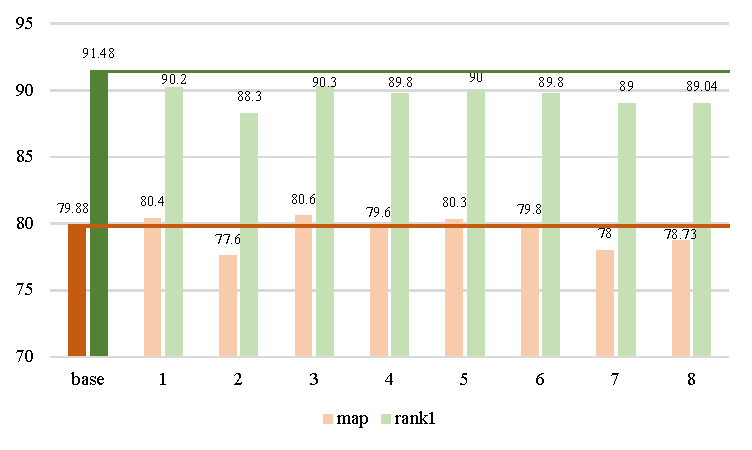
\includegraphics[width=\linewidth]{figs/pdf/samepose.pdf}
\caption{ReID results with images generated with the same pose on Market1501.}
\label{fig:samepose}
\end{figure}

\begin{figure}
\centering
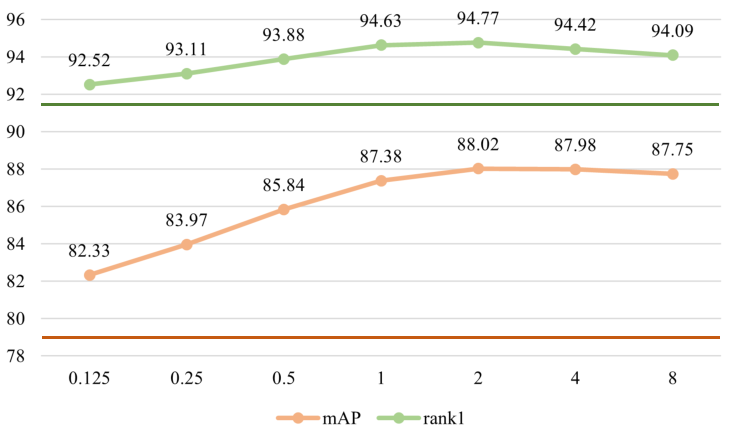
\includegraphics[width=0.9\linewidth]{figs/pdf/eta.pdf}
\caption{Impact of the quality coefficient \( \eta \) with TransReID on Market1501. The dark color lines are the baseline.}
\label{fig:eta}
\end{figure}

\begin{figure}
\centering
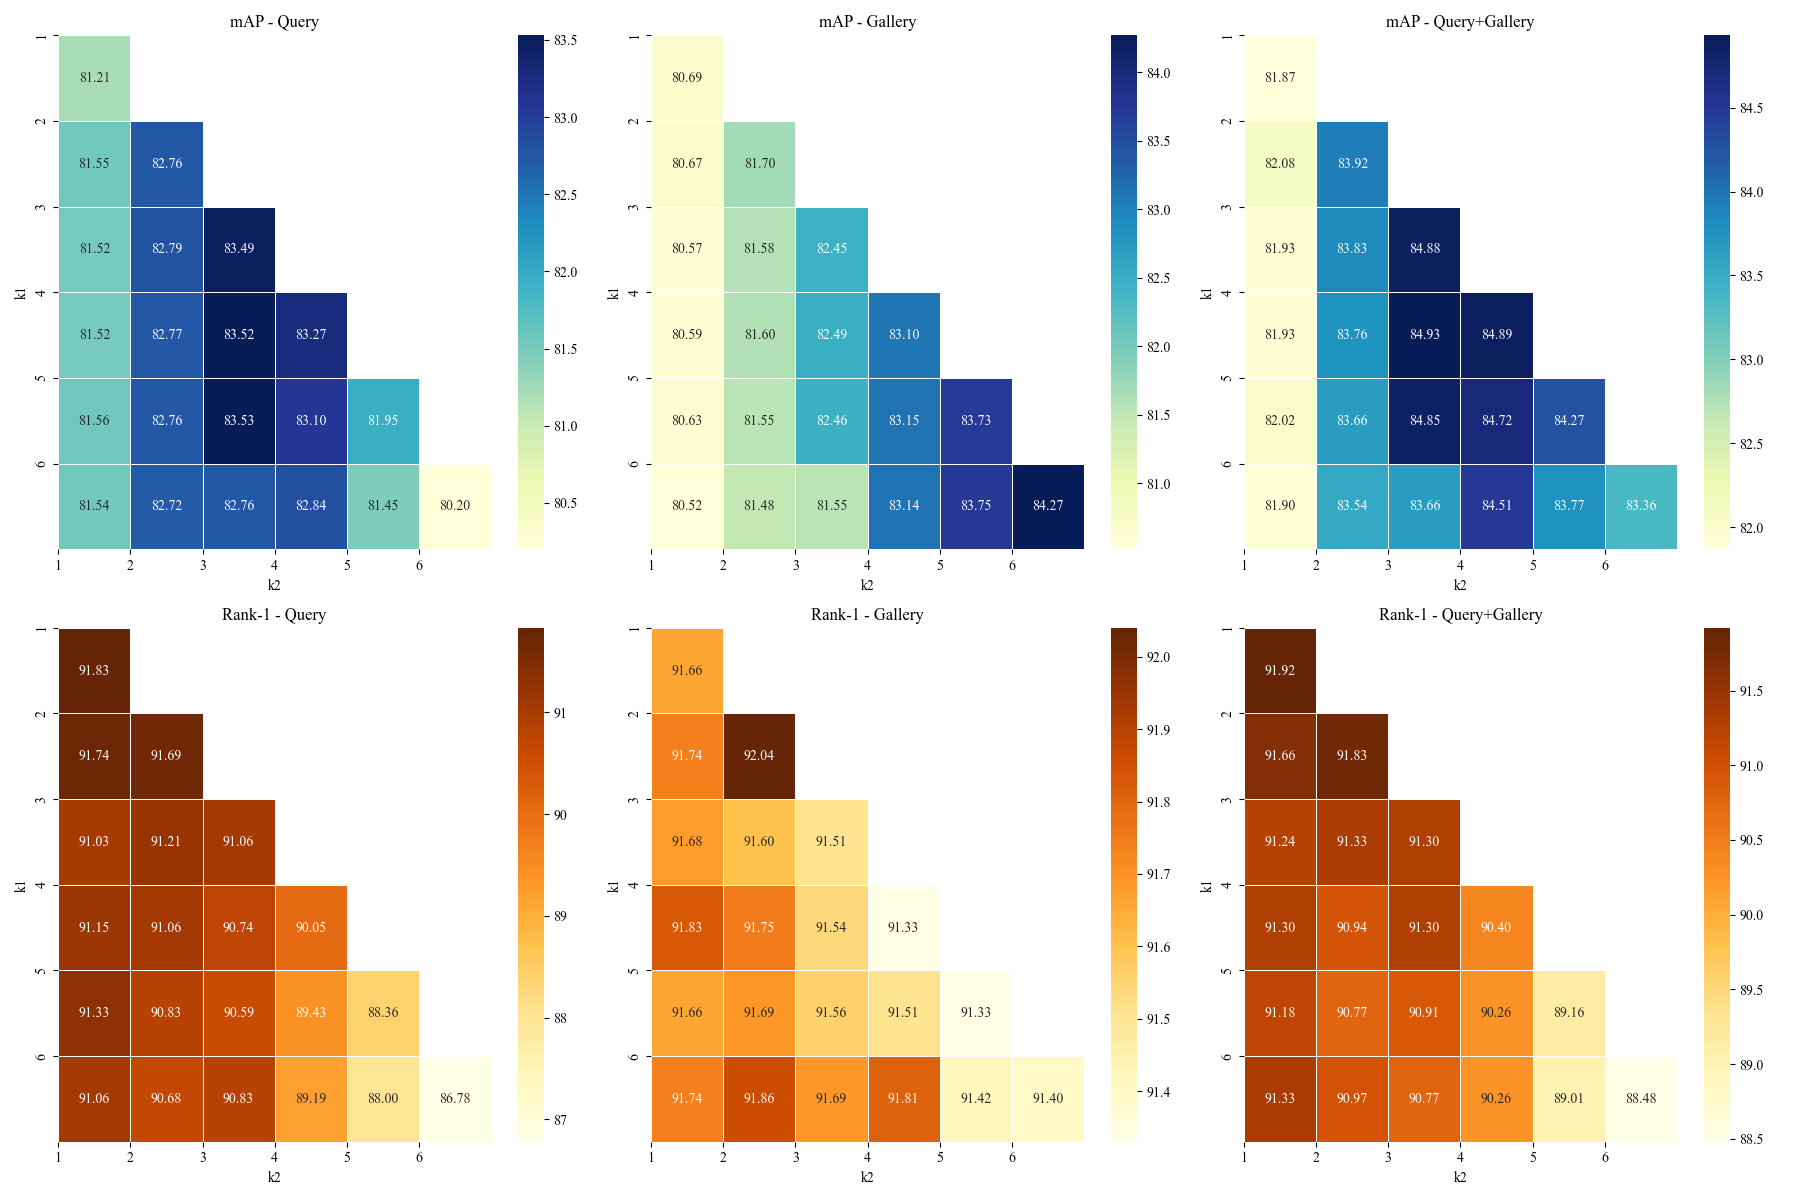
\includegraphics[width=0.9\linewidth]{figs/k1k2.png}
\caption{$k_1/k_2$ analysis of Neighbor Feature Centralization (NFC) with TransReID on Market1501 without re-ranking.}
\label{fig:k1k2}
\end{figure}

\section{Experiments Supplementary}
\begin{figure*}
\centering
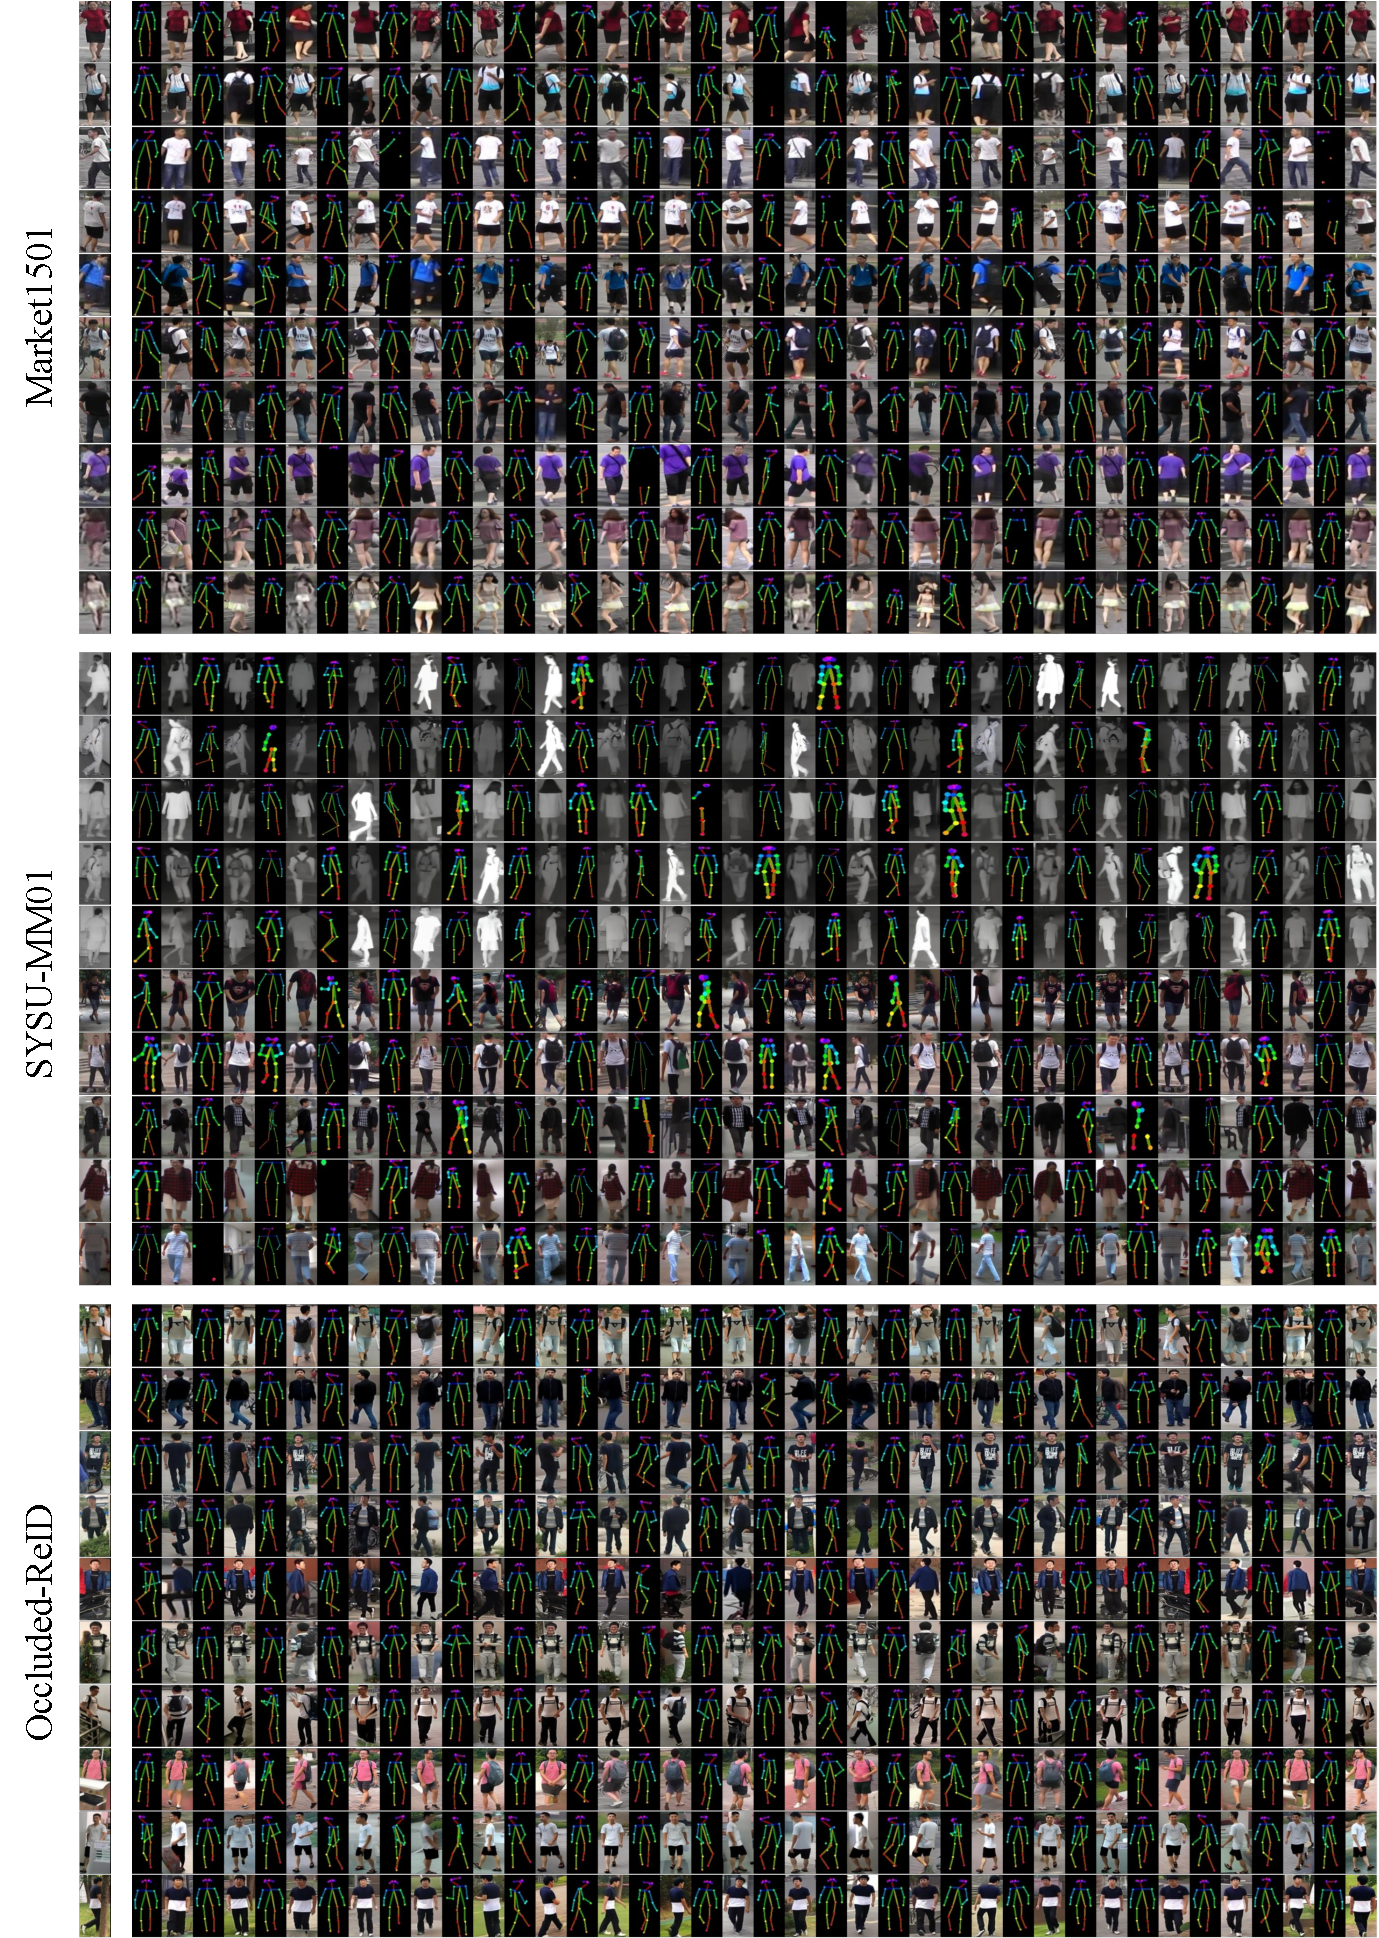
\includegraphics[width=\linewidth]{figs/pdf/random_l.pdf}
\caption{More random generated images on three datasets.}
\label{fig:random_all}
\end{figure*}
\subsection{Data Cleansing}
Training an effective generative model requires high-quality data support. In current ReID (Person Re-Identification) datasets, there are many low-quality images, and removing them can help reduce interference to the model. In our experiments, we found two main issues that need to be addressed: \textbf{Extremely Low-quality Images}: The dataset contains images with such low resolution that even the human eye cannot recognize them as a "person". \textbf{Pose Estimation Failures}: The pose estimation model inevitably fails to detect pedestrian poses in some images.

\subsubsection{Extremely Low-quality Images}

To address this, manual filtering is impractical. Therefore, we designed an automated filtering algorithm. We leverage normal distribution of feature vector, if the feature on the edge of the distribution, largely due to the data itself is out of the distribution of its identity, and it can be picked up. 
% We calculate the mean and covariance matrix of the feature vectors for each ID and filter out samples whose feature distances lie outside a predefined quantile range.

Let \( \mathbf{f}_i \in \mathbb{R}^d \) denote the feature vector of the \( i \)-th sample of a particular identity, where \( d \) is the feature dimension. The mean vector \( \boldsymbol{\mu} \) and covariance matrix \( \boldsymbol{\Sigma} \) are computed as follows:
\begin{equation} 
\boldsymbol{\mu} = \frac{1}{N} \sum_{i=1}^{N} \mathbf{f}_i, \quad \boldsymbol{\Sigma} = \frac{1}{N} \sum_{i=1}^{N} (\mathbf{f}_i - \boldsymbol{\mu})(\mathbf{f}_i - \boldsymbol{\mu})^\top
\end{equation}
where \( N \) is the number of samples for a given ID.

To detect outliers, we compute the Mahalanobis distance \( d_i \) of each feature vector \( \mathbf{f}_i \) from the mean vector \( \boldsymbol{\mu} \), defined as:
\begin{equation}
dis_i = \sqrt{ (\mathbf{f}_i - \boldsymbol{\mu})^\top \boldsymbol{\Sigma}^{-1} (\mathbf{f}_i - \boldsymbol{\mu}) }
\end{equation}

Given that the feature vectors are assumed to follow a multivariate normal distribution, we use quantiles of the Mahalanobis distance to filter out outliers. Specifically, we define a lower bound \( Q_p \) and an upper bound \( Q_{1-p} \) based on the \( p \)-th and \( (1 - p) \)-th quantiles, respectively. Samples with distances outside this range are considered outliers and are removed, and can get a set $S^{\text{ref}}_{i}$ for $i^{th}$ ID:
\begin{equation} \label{outliers}
S_i^{\text{ref}} = \{ \mathbf{x}_i \mid dis_i \in [Q_p, Q_{1-p}] \}
\end{equation}



\begin{figure}
\centering
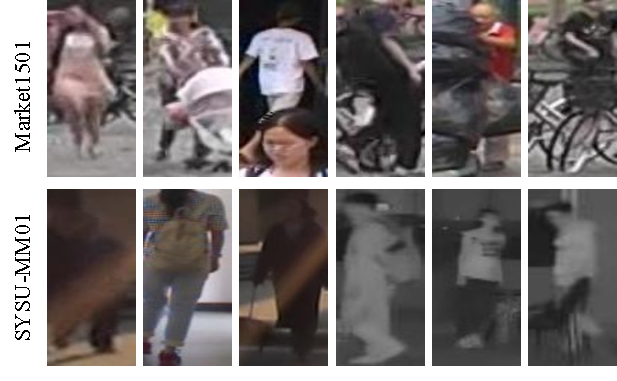
\includegraphics[width=0.8\linewidth]{figs/pdf/outliers.pdf}
\caption{Some outliers detected via the mechanism formulated as Equation.\ref{outliers} on Market1501 and SYSU-MM01 with quartile 0.005.}
\label{fig:outliers}
\end{figure}


\subsubsection{Pose Filtering for 'Failed' Pose Estimation}
\label{PoseValid}
We designed a pose filtering algorithm called PoseValid to eliminate cases where pose extraction has "completely failed." This algorithm checks the validity of the pose keypoints based on factors such as occlusion, keypoint positions, angles, and limb proportions, then get the set of valid poses.
\begin{equation}
S^{\text{trg}}_i = \{ \mathbf{x}_i \mid \text{PoseValid}(\mathbf{x}_i) \text{ and } dis_i \in [Q_p, Q_{1-p}] \}
\end{equation}
where the pose detector in this paper uses pretrained model of DWpose\cite{yang2023effective}. Given a set of keypoints representing a pose, we normalize the pose using the following steps:
\begin{enumerate}
    \item Compute the body height ($h$):\\
    Calculate the Euclidean distance between the Neck (keypoint 1) and the Left Hip (keypoint 11):
    \[
    h = \left\| \mathbf{k}_{\text{Neck}} - \mathbf{k}_{\text{LHip}} \right\|
    \]
    \item Translate the pose:\\
    Shift all keypoints so that the Neck is at the origin:
    \[
    \mathbf{k}'_i = \mathbf{k}_i - \mathbf{k}_{\text{Neck}}
    \]
    \item Scale the pose:\\
    Divide each keypoint by the body height to normalize the size:
    \[
    \mathbf{k}^{\text{normalized}}_i = \frac{\mathbf{k}'_i}{h}
    \]
\end{enumerate}
Then, the filtering process of PoseValid function evaluates the validity of pose keypoints by applying constraints on limb lengths, symmetry, and keypoint positions. 

\subsection{Generation quality and Pose Representation Study}
To assess the quality of the generated images, we replaced the real images in the dataset with images of the same pose and performed inference validation. The results, as shown in Fig.\ref{fig:samepose}, indicate that the original model still successfully matches pedestrians without significant performance degradation. Even with all images in the same pose, the model can effectively differentiate between individuals. This suggests that our generated images are of high quality, retaining the main characteristics of the original images without notably impacting the ReID model. Moreover, we found that pedestrians walking at an angle have higher distinguishability compared to other poses (front, back, and side views), which are more representative of their identities.


\begin{table}[]
\small
\renewcommand{\arraystretch}{1.0}
\renewcommand\tabcolsep{5pt}
\centering
    \begin{tabular}{cc|ccc}
        \hline
        +Ours & +Rerank & mAP & Rank1  \\ \hline
        \ding{55} &\ding{55} & 79.88 & 91.48 \\
        \ding{55} &\ding{51} & 89.56 & 92.07  \\ \hline
        \rowcolor{gray!20}
        \ding{51} &\ding{55} &90.39&94.74\\
        \rowcolor{gray!20}
        \ding{51} &\ding{51}  & \textbf{92.79}&	\textbf{94.83} \\ \hline
    \end{tabular}
    \caption{Compared to k-reciprocal rerank with official settings on Market1501 ($k_1$=20,$k_2$=6).}
    \label{tab:rerank}
\end{table}

\begin{table}[]
\small
\renewcommand{\arraystretch}{1.0}
\renewcommand\tabcolsep{5pt}
\centering
        \begin{tabular}{c|ccc}
        \hline
        Methods & mAP & Rank1  \\ \hline
        TransReID on MSMT17 & 67.80	&85.33\\
        \rowcolor{gray!20}
        +ours & 74.06	&86.55	  \\ \hline
    \end{tabular}
    \caption{Experiment on MSMT17 with TransReID and their official weights.}
    \label{tab:more}
\end{table}


\subsection{More Random Generation}
We provide additional randomly generated images in Fig.\ref{fig:random_all} from Market-1501, SYSU-MM01 and Occluded-ReID datasets.


\subsection{Collaborate with Re-ranking}
Since our method does not change the features' original distribution,
it could collaborate post-processing strategies like rerank, as shown in Tab.\ref{tab:rerank}.

\subsection{Results on MSMT17 with TransReID}
We conduct a simple experiment on MSMT17 dataset with with TransReID and their official pre-trained weights. As shown in Tab.\ref{tab:more}.

\subsection{Comparisons with state-of-the-art methods on three ReID benchmarks}
Comparison on three ReID benchmarks. Since Our method can be applied to any baseline, we choose three methods from three benchmarks which have the official codes and pre-trained weights. With our method, we achieve the new SOTA in three benchmarks, as shown in Fig.\ref{tab:sota_m} and Fig.\ref{tab:sys}.



\begin{table}
\centering
\renewcommand\tabcolsep{5pt}

\begin{tabular}{c|cc|cc}
\hline
 \multirow{2}{*}{Methods}& \multicolumn{2}{c|}{Market1501} & \multicolumn{2}{c}{Occluded-reID} \\ \cline{2-5}
 & Rank-1 & mAP & Rank-1  & mAP \\
\hline
BoT\cite{luo2019bag} & 94.5 & 85.9 & 58.4 & 52.3 \\
PCB\cite{sun2018beyond}& 93.8 & 81.6& - & - \\
VGTri\cite{yang2021learning} & - & - & 81.0 & 71.0 \\
PVPM\cite{gao2020pose} & - & - & 66.8 & 59.5 \\
HOReID\cite{wang2020high} & 94.2 & 84.9 & 80.3 & 70.2 \\
ISP\cite{zhu2020identity} & 95.3 & 88.6 & - & -\\
PAT\cite{li2021diverse} & 95.4 & 88.0 & 81.6 & 72.1 \\
TRANS\cite{he2021transreid} & 95.2 & 88.9 & - & - \\
CLIP\cite{li2023clip} & 95.7 & 89.8 & - & - \\
SOLIDER\cite{chen2023beyond} & 96.9 & 93.9 & - & - \\
SSGR\cite{yan2021occluded} & 96.1 & 89.3 & 78.5 & 72.9 \\
FED\cite{wang2022feature} & 95.0 & 86.3& 86.3 & 79.3 \\
BPBreid\cite{somers2023body} & 95.7 & 89.4 & 82.9 & 75.2\\
PFD\cite{wang2022pose} & 95.5 & 89.7 & 83.0 & 81.5 \\
KPR\textsubscript{IN}\cite{somers2025keypoint} & 95.9 & 89.6 & 85.4 & 79.1 \\
KPR\textsubscript{SOL}\cite{somers2025keypoint} & 96.62 &93.22 &84.83& 82.6\\
\hline
\rowcolor{gray!20}
CLIP+ours & 97.3 & 94.9 & - & -\\
\rowcolor{gray!20}
KPR\textsubscript{IN}+ours & - & - & 91 & 89.34 \\
\hline
\end{tabular}
\caption{Comparisons with state-of-the-art methods on Market1501 and Occluded-reID.}
\label{tab:sota_m}
\end{table}
\begin{table}
\small
\centering
% \renewcommand{\arraystretch}{1.1}
\renewcommand\tabcolsep{5pt}
	\begin{tabular}{l|cc|cc}
		\hline
		\multirow{2}{*}{Methods} & \multicolumn{2}{c|}{All-Search} &\multicolumn{2}{c}{Indoor-Search}\\ \cline{2-5}
              & mAP & Rank-1 & mAP & Rank-1 \\ \cline{1-5}
             PMT\cite{lu2023learning}& 66.13& 67.70& 77.81& 72.95\\
             MCLNet~\cite{hao2021cross}& 61.98 &65.40&76.58 &72.56\\
             MAUM~\cite{Liu2022LearningMU}& 68.79 &71.68& 81.94 &76.9\\
             CAL\cite{CAL}& 71.73 &74.66& 83.68 &79.69\\
             SAAI(w/o AIM)~\cite{fang2023visible}&  71.81& 75.29&  84.6 &81.59\\
             SEFL\cite{feng2023shape}& 72.33 &77.12& 82.95 &82.07\\
             PartMix\cite{kim2023partmix}& 74.62 &77.78& 84.38 &81.52\\
             MID~\cite{Huang2022ModalityAdaptiveMA} & 59.40 &60.27& 70.12 &64.86\\
             FMCNet~\cite{zhang2022fmcnet}& 62.51 &66.34& 74.09 &68.15\\
             MPANet~\cite{wu2021discover}& 68.24 &70.58& 80.95 &76.74\\
             CMT~\cite{jiang2022cross}& 68.57 &71.88& 79.91 &76.90\\
             protoHPE~\cite{zhang2023protohpe}& 70.59 &71.92&81.31 &77.81\\
             MUN~\cite{yu2023modality}& 73.81 &76.24& 82.06 &79.42\\
             MSCLNet~\cite{zhang2022modality}& 71.64 &76.99& 81.17 &78.49\\
             DEEN~\cite{zhang2023diverse}& 71.80 &74.70& 83.30 &80.30\\
             CIFT~\cite{li2022counterfactual}& 74.79 &74.08& 85.61 &81.82\\
             \cline{1-5}
             \rowcolor{gray!20}
            SAAI+ours&76.44&79.33& 86.83& 84.2\\
             \cline{1-5}
	\end{tabular}
             \caption{Comparison with state-of-the-art methods on SYSU-MM01 without re-ranking.}
             \label{tab:sys}                               
\end{table}


% \begin{figure*}
% \centering
% 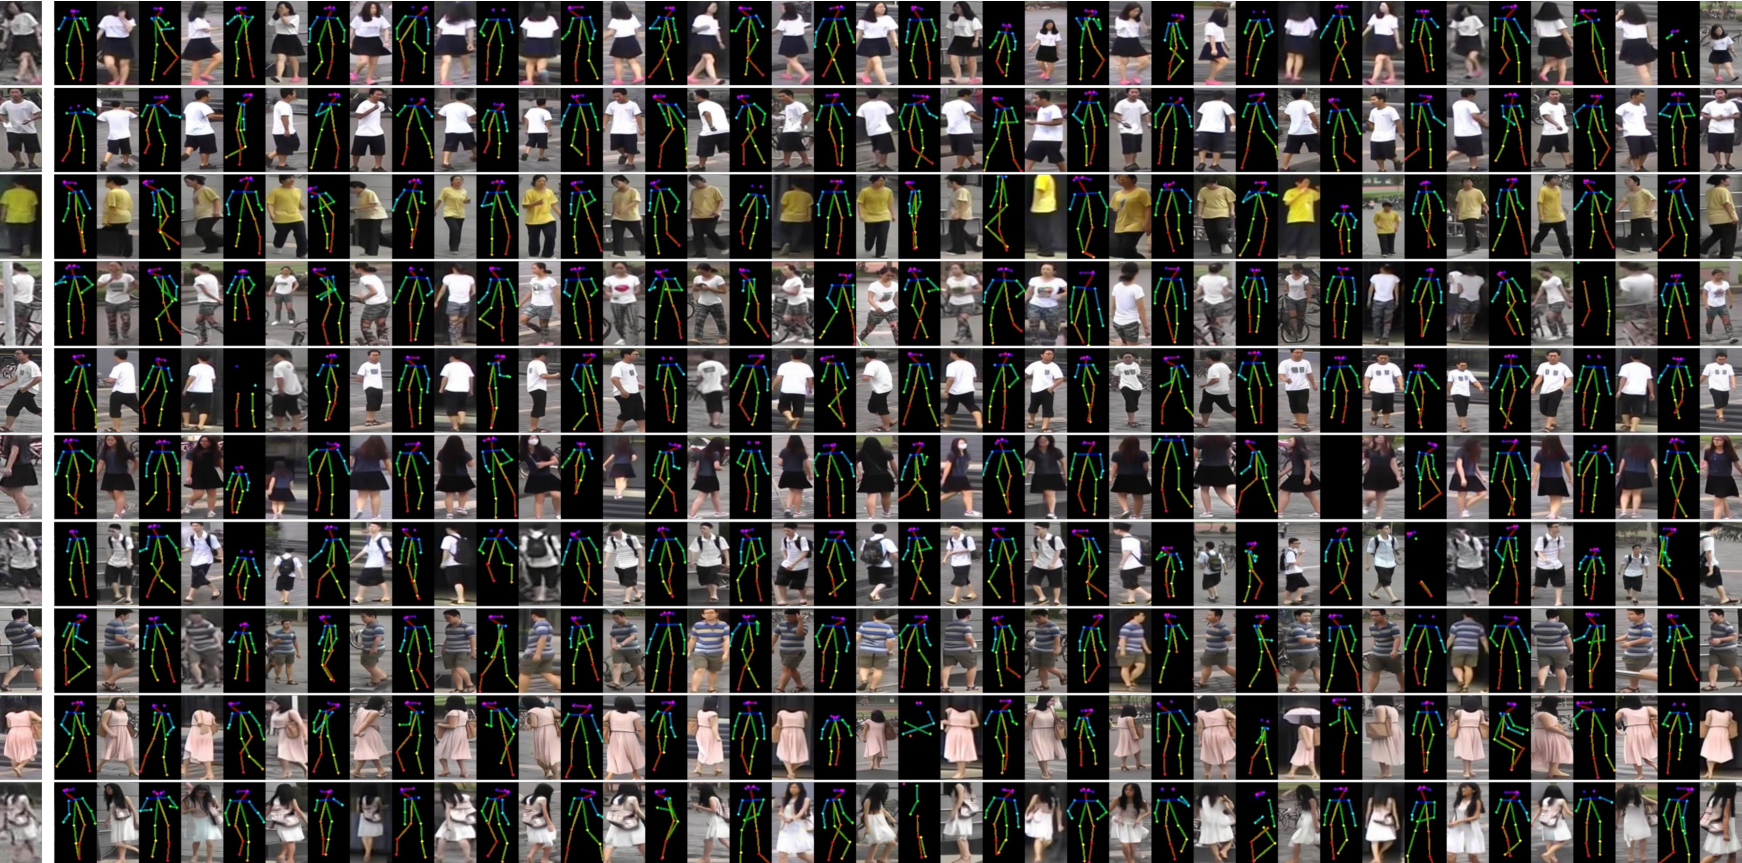
\includegraphics[width=\linewidth]{figs/pdf/random.pdf}
% \caption{Random generated images on Market1501.}
% \label{fig:random_market}
% \end{figure*}

% \begin{figure*}
% \centering
% \includegraphics[width=\linewidth]{figs/pdf/sysu.pdf}
% \caption{Random generated images on SYSU-MM01.}
% \label{fig:random_sysu}
% \end{figure*}


% \begin{figure*}
% \centering
% \includegraphics[width=\linewidth]{figs/pdf/occ.pdf}
% \caption{Random generated images on SYSU-MM01.}
% \label{fig:random_occ}
% \end{figure*}


\subsection{Analysis on quality coefficient $\eta$ of Generation Model}

Fig.\ref{fig:eta} illustrates the effect of adjusting the coefficient $\eta$ on the performance of the ReID model. To evaluate this impact, we gradually increased the value of $\eta$ and observed changes on the mAP and Rank-1 metrics. 

As the value of $\eta$ increases, the performance of the ReID model improves, reaching an optimal point. At $\eta = 2$, both mAP and Rank-1 achieve their maximum values of 88.02\% and 94.77\%, respectively. However, further increasing $\eta$ beyond this point leads to a slight decline in performance. It is easy to find that using generated images to centralize features is effective. However, considering the quality of the generated image, direct adding, although also effective, may not always achieve the best results. Therefore adjusting $\eta$ according to the generation quality of the model in this dataset can better centralize the features.


\subsection{Analysis on $k_1/k_2$ of Neighbor Feature Centralization}
We conducted a detailed analysis of different $k_1$ and $k_2$ combinations, evaluating the results of feature centralization enhancement separately on the Query and Gallery sets, as well as the combined effect (as shown in the Fig.\ref{fig:k1k2}). The selection of these two parameters primarily depends on the number of potential positive samples within the set (adjusting $k_1$) and the confidence in feature associations (adjusting k2). Overall, medium parameter combinations ($k_1$ and $k_2$ in the range of 2-4) provide relatively optimal performance.




























% \begin{equation}
% \mathbf{E}_{i+1} = \text{SiLU}(\text{Conv}_{i, \text{stride}=2}(\text{Conv}_{i}(\mathbf{E}_i)))
% \end{equation}
% \paragraph{Forward Process}

% The Denoising Diffusion Implicit Model (DDIM) \cite{song2020denoising} is fundamental to our approach. The forward process gradually adds Gaussian noise to the data:
% \begin{equation}
% q(\mathbf{z}_t \mid \mathbf{z}_{t-1}) = \mathcal{N}(\mathbf{z}_t; \sqrt{\alpha_t} \mathbf{z}_{t-1}, (1 - \alpha_t) \mathbf{I})
% \end{equation}
% where \( \alpha_t \) controls the noise schedule, and \( \mathbf{z}_t \) is the noisy latent at timestep \( t \).

% \paragraph{Reverse Process}

% The model learns to reverse the diffusion process with classifier-free guidance \cite{ho2022classifier}:
% \begin{equation}
% \begin{aligned}
%     \mathbf{z}_{t-1} &= \boldsymbol{\mu}(\mathbf{z}_t, t, \mathbf{E}_{\text{pose}}, \mathbf{H}) - w \cdot (\hat{\boldsymbol{\epsilon}}^{\text{cond}} - \hat{\boldsymbol{\epsilon}}^{\text{uncond}}) \\
%     \hat{\boldsymbol{\epsilon}}^{\text{cond}} &= \boldsymbol{\epsilon}_{\theta}(\mathbf{z}_t, t, \mathbf{E}_{\text{pose}}, \mathbf{H}) \\
%     \hat{\boldsymbol{\epsilon}}^{\text{uncond}} &= \boldsymbol{\epsilon}_{\theta}(\mathbf{z}_t, t, \mathbf{E}_{\text{pose}}, \mathbf{H} = 0)
% \end{aligned}
% \end{equation}

% The model predicts the mean \( \boldsymbol{\mu} \) of the posterior distribution at each timestep, conditioned on the pose features and conditioning embedding.
% \begin{equation}
% \small
% \boldsymbol{\mu}(\mathbf{z}_t, t, \mathbf{E}_{\text{pose}}, \mathbf{H}) = \frac{1}{\sqrt{\alpha_t}} \left( \mathbf{z}_t - \frac{1 - \alpha_t}{\sqrt{1 - \bar{\alpha}_t}} \boldsymbol{\epsilon}_{\theta}(\mathbf{z}_t, t, \mathbf{E}_{\text{pose}}, \mathbf{H}) \right)
% \end{equation}
% \( \hat{\boldsymbol{\epsilon}} \) is the predicted noise by the denoising UNet, and \( \bar{\alpha}_t = \prod_{s=1}^{t} \alpha_s \).
{
    \small
    \bibliographystyle{ieeenat_fullname}
    \bibliography{main}
}

% WARNING: do not forget to delete the supplementary pages from your submission 
% \setcounter{section}{0}
\clearpage
\setcounter{page}{1}
\maketitlesupplementary



\section{Methods Supplementary}
\subsection{Aggregation role of ReID loss functions}
Currently, ReID models commonly use cross-entropy loss to impose ID-level constraints, and contrastive losses (such as triplet loss) to bring features of the same ID closer while pushing apart features of different IDs. Some models also utilize center loss to construct identity centers for dynamically constraining the IDs. These methods lead to one common result: feature aggregation. From the perspective of the gradient of the loss functions, we could prove that the feature vectors of each ID in current ReID tasks naturally aggregate around a center or mean in the followings.
\paragraph{Cross-Entropy Loss} 
is often used in classification tasks, optimizing the model by maximizing the probability of the correct class. Given $N$ samples, each with a feature vector $\mathbf{z}_i \in \mathbb{R}^d$, and its corresponding class label $y_i \in \{1, 2, \dots, C\}$, the cross-entropy loss is defined as:
\begin{equation}
\mathcal{L}_{\text{CE}} = -\frac{1}{N} \sum_{i=1}^{N} \log \frac{\exp(\mathbf{w}_{y_i}^\top \mathbf{z}_i + b_{y_i})}{\sum_{j=1}^{C} \exp(\mathbf{w}_j^\top \mathbf{z}_i + b_j)}
\end{equation}
where $\mathbf{w}_j$ and $b_j$ are the weight vector and bias for class $j$, respectively.

For simplicity, assume that the final layer is a linear classifier without bias, i.e., $b_j = 0$. When the loss is minimized, the optimization objective is to maximize the score $\mathbf{w}_{y_i}^\top \mathbf{z}_i$ of the correct class while minimizing the scores $\mathbf{w}_j^\top \mathbf{z}_i$ of other classes ($j \neq y_i$).

By gradient descent optimization, we can obtain:
\begin{equation}
\frac{\partial \mathcal{L}_{\text{CE}}}{\partial \mathbf{z}_i} = 1/N\left(p_{y_i} - 1\right) \mathbf{w}_{y_i} + 1/N\sum_{j \neq y_i} p_{ij} \mathbf{w}_j
\end{equation}
where $p_{ij} = \frac{\exp(\mathbf{w}_j^\top \mathbf{z}_i)}{\sum_{k=1}^{C} \exp(\mathbf{w}_k^\top \mathbf{z}_i)}$.

With the loss function converges, $p_{y_i}\rightarrow1$ and $p_{ij}\rightarrow0 (j \neq y_i)$. The feature $\mathbf{z}_i$ is optimized to be near a linear combination of the class weight vectors $\mathbf{w}_{y_i}$. This indicates that features of the same class will tend toward a common direction, thus achieving feature aggregation.

\paragraph{Contrastive loss} (Triplet Loss as example) optimizes the feature space by bringing samples of the same class closer and pushing samples of different classes further apart. A triplet $(\mathbf{z}_a, \mathbf{z}_p, \mathbf{z}_n)$ is defined, where $\mathbf{z}_a$ is the anchor, $\mathbf{z}_p$ is the positive sample (same class), and $\mathbf{z}_n$ is the negative sample (different class). The triplet loss is defined as:
\begin{equation}
\mathcal{L}_{\text{Triplet}} = \max \left( \| \mathbf{z}_a - \mathbf{z}_p \|_2^2 - \| \mathbf{z}_a - \mathbf{z}_n \|_2^2 + \alpha, 0 \right)
\end{equation}
where $\alpha$ is the margin parameter.

To minimize the loss, the optimization objective is:
\begin{equation}
\| \mathbf{z}_a - \mathbf{z}_p \|_2^2 + \alpha < \| \mathbf{z}_a - \mathbf{z}_n \|_2^2
\end{equation}
\begin{align}
\frac{\partial \mathcal{L}_{\text{Triplet}}}{\partial \mathbf{z}_a} &= 2 (\mathbf{z}_n - \mathbf{z}_p), \\
\frac{\partial \mathcal{L}_{\text{Triplet}}}{\partial \mathbf{z}_p} &= 2 (\mathbf{z}_p - \mathbf{z}_a), \\
\frac{\partial \mathcal{L}_{\text{Triplet}}}{\partial \mathbf{z}_n} &= 2 (\mathbf{z}_a - \mathbf{z}_n).
\end{align}

By minimizing triplet loss, the feature $\mathbf{z}_p$ is pulled closer to $\mathbf{z}_a$, while $\mathbf{z}_n$ is pushed away. Through this mechanism, Triplet Loss encourages features of the same class to aggregate together while features of different classes are separated from each other.

\paragraph{Center loss} further enhances feature aggregation by introducing a feature center for each class. For each class $j$, there is a feature center $\mathbf{c}_j$, and the center loss is defined as:
\begin{equation}
\mathcal{L}_{\text{Center}} = \frac{1}{2} \sum_{i=1}^{N} \| \mathbf{z}_i - \mathbf{c}_{y_i} \|_2^2
\end{equation}

The goal of minimizing center loss is to make each sample's feature vector $\mathbf{z}_i$ as close as possible to its corresponding class center $\mathbf{c}_{y_i}$. Through gradient descent, we obtain:
\begin{align}
\frac{\partial \mathcal{L}_{\text{Center}}}{\partial \mathbf{z}_i} &= \mathbf{z}_i - \mathbf{c}_{y_i} \\
\frac{\partial \mathcal{L}_{\text{Center}}}{\partial \mathbf{c}_j} &= \begin{cases}
\mathbf{c}_j - \mathbf{z}_i & \text{if } y_i = j \\
0 & \text{otherwise}
\end{cases}
\end{align}

Thus, the optimization process not only pulls sample features closer to their centers but also dynamically updates each class's center to represent the mean of that class's feature distribution. This directly encourages features of the same class to aggregate together.



% \paragraph{Limb Length Constraints}

% Let \( \mathbf{k}_i = (x_i, y_i) \) represent the normalized coordinates of the \( i \)-th keypoint in the image. The Euclidean distance between two keypoints \( \mathbf{k}_i \) and \( \mathbf{k}_j \), corresponding to body joints, is given by:
% \begin{equation}
% d(\mathbf{k}_i, \mathbf{k}_j) = \sqrt{(x_i - x_j)^2 + (y_i - y_j)^2}
% \end{equation}

% For example, the length of the left arm, denoted as \( d_{\text{left arm}} \), is calculated as the distance between the left shoulder and left elbow keypoints:
% \begin{equation}
% d_{\text{left arm}} = d(\mathbf{k}_{\text{LS}}, \mathbf{k}_{\text{LE}})
% \end{equation}
% \begin{equation}
% d_{\text{right arm}} = d(\mathbf{k}_{\text{RS}}, \mathbf{k}_{\text{RE}})
% \end{equation}

% We ensure that limb lengths fall within a reasonable range, defined by the minimum and maximum allowable limb lengths:
% \begin{equation}
% l_{\text{min}} \leq d_{\text{left arm}}, d_{\text{right arm}}, d_{\text{left leg}}, d_{\text{right leg}} \leq l_{\text{max}}
% \end{equation}


% \paragraph{Positional Constraints}

% Finally, we apply positional constraints to ensure keypoints are in anatomically plausible positions. For example, the head \( \mathbf{k}_{\text{H}} \) must be higher than the center of the body \( \mathbf{k}_{\text{C}} \) and the knees must be positioned below the hips:
% \begin{equation}
% y_{\text{H}} < y_{\text{C}}
% \end{equation}
% \begin{equation}
% y_{\text{LK}} > y_{\text{LH}}, \quad y_{\text{RK}} > y_{\text{RH}}
% \end{equation}

% \subsubsection{Identity Feature Redistribution}

% We use the pretrained ReID model to extract identity features:
% \begin{equation}
% \mathbf{f} = \text{ReID}(\mathbf{x}^{\text{ref}})
% \end{equation}

% On this basis, we design a learnable Feature Re-Distribution mapping module (IFR) to allow the model to optimize the feature distribution $\mathbf{f} \in \mathbb{R}^d$ while reducing the interference of feature noise on the diffusion model. Then use this as the conditioning embedding \( \mathbf{H} \in \mathbb{R}^{N \times D} \):
% \begin{equation}
% \mathbf{H} = \text{IFR}(\mathbf{f})
% \end{equation}

% The ReID Prompt Module projects and concatenates the features:
% \begin{align}
% \mathbf{h} &= \text{Linear}_{\text{ReID}}(\mathbf{f}) \in \mathbb{R}^{N \times D} \\
% \mathbf{H} &= \text{LayerNorm}(\mathbf{h})
% \end{align}
% where \( N \) is the sequence length, and \( D \) is the feature dimension.




\subsection{Identity Density ($\text{ID}^2$) Metric}
Identity density is one aspect of measuring ReID effectiveness. However, there is currently no quantitative metric for this, and researchers commonly rely on visualization tools like t-SNE to demonstrate model performance. Due to the large number of IDs, this approach is limited to visualizing only a few IDs, making it challenging to assess model performance from a global perspective quantitatively. Some researchers exploit this limitation by selecting the best-performing IDs of their models for visualization. To address this, we propose an Identity Density ($\text{ID}^2$) Metric. This metric evaluates the global ID aggregation performance by taking each ID center across the entire test set (gallery and query) as a benchmark.
\begin{equation}
\text{ID}^2 = \frac{1}{N} \sum_{i=1}^{N} \frac{1}{n_i} \sum_{j=1}^{n_i} d\left( \frac{f_{ij}}{\|f_{ij}\|_2}, c_i \right)
\end{equation}
where \( N \) is the total number of unique IDs in the test set, and \( n_i \) is the number of samples for ID \( i \). The feature vector of the \( j \)-th sample of ID \( i \) is denoted as \( f_{ij} \), and \( c_i \) represents the identity center of ID \( i \), computed as follows:
\begin{equation}
c_i = \frac{1}{n_i} \sum_{j=1}^{n_i} \frac{f_{ij}}{\|f_{ij}\|_2}
\end{equation}

Both the feature vectors \( f_{ij} \) and the identity centers \( c_i \) are \( L_2 \)-normalized to ensure consistent feature scaling. The function \( d(\cdot, \cdot) \) represents the Euclidean distance. 


\subsection{Pose Encoder Details}

The Pose Encoder module is designed to extract high-dimensional pose embeddings from the input poses. 
\begin{equation}
\mathbf{E}_{\text{pose}} = \text{PoseEncoder}(\mathbf{x}^{\text{pose}})
\end{equation}

The input is a feature map of size \(C_{\text{in}} \times H \times W\), denoted as \( \mathbf{x}^{\text{pose}} \), 
where \(C_{\text{in}}\) is the number of input channels, and \(H, W\) are the height, and width of the input. 
The first convolution layer is defined as:
\begin{equation}
\mathbf{E}_0 = \text{SiLU}(\text{Conv}_{\text{in}}(\mathbf{x}^{\text{pose}}))
\end{equation}
where \( \text{Conv}_{\text{in}} \) is a convolution operation with kernel size \(3 \times 3\), 
and the number of channels changes from \( C_{\text{in}} =3\) to \( C_0 =16\):

Each block applies a normal \(3 \times 3\) Conv, a \(3 \times 3\) Conv with stride 2 to reduce spatial dimensions, and followed by a SiLU activate function.
For the \(i\)-th convolutional block, the operations can be expressed as:
\begin{equation}
\mathbf{E}_{i+1} = \text{SiLU}(\text{Conv}_{i, \text{stride}=2}(\text{Conv}_{i}(\mathbf{E}_i)))
\end{equation}

The number of channels for each block is as follows: $[C_0, C_1, C_2, C_3] = [16, 32, 64, 128]$

The output Conv layer maps the features from the last block to the target embedding dimension \(C_{\text{out}} = 320\), 
expressed as:
\begin{equation}
\mathbf{E}_{\text{pose}} = \text{Conv}_{\text{out}}(\mathbf{E}_4)
\end{equation}


\subsection{Detailed Description of Neighbor Feature Centralization (NFC)}

\paragraph{Step 1: Compute Distance Matrix}

Given all feature vectors in the gallery \(\{\mathbf{z}_i\}_{i=1}^N\), our goal is to enhance each feature vector by aggregating features from its mutual nearest neighbors.
Compute the pairwise distance matrix \(\mathbf{D} = [d_{ij}]\) where \(d_{ij}\) represents the distance between features \(\mathbf{z}_i\) and \(\mathbf{z}_j\). To avoid self-matching, set the diagonal elements to a large constant, i.e. \[d_{ii} = C, \quad \text{for } i = 1, 2, \dots, N\]

\paragraph{Step 2: Find Top \(k_1\) Nearest Neighbors}

For each feature \(\mathbf{z}_i\), find its top \(k_1\) nearest neighbors based on the distance matrix \(\mathbf{D}\). Denote the set of indices of these neighbors as:
\begin{equation}
\mathcal{N}_{i} = \operatorname{TopK}_{k_1}(\{d_{ij}\}_{j=1}^N)
\end{equation}

\paragraph{Step 3: Identify Mutual Nearest Neighbors}

For each feature \(\mathbf{z}_i\), identifies its mutual nearest neighbors by checking whether each neighbor in \(\mathcal{N}_{i}\) also considers \(\mathbf{z}_i\) as one of its top \(k_2\) nearest neighbors. Specifically, for each \(j \in \mathcal{N}_{i}\), checks if \(i \in \mathcal{N}_{j}^{k_2}\), where \(\mathcal{N}_{j}^{k_2}\) is the set of indices of the top \(k_2\) nearest neighbors of \(\mathbf{z}_j\). If this condition is satisfied, add \(j\) to the mutual nearest neighbor set \(\mathcal{M}_{i}\):
\begin{equation}
\mathcal{M}_{i} = \{ j \mid j \in \mathcal{N}_{i}, \, i \in \mathcal{N}_{j}^{k_2} \}
\end{equation}

\paragraph{Step 4: Feature Centralization Enhancement}

Then it could centralize each feature vector \(\mathbf{z}_i\) by aggregating the features of its mutual nearest neighbors:
\begin{equation}
\mathbf{z}_i^{\text{centralized}} = \mathbf{z}_i + \sum_{j \in \mathcal{M}_{i}} \mathbf{z}_j
\end{equation}

This aggregation reduces feature noise and improves discriminability by incorporating information from similar features.

\begin{figure}
\centering
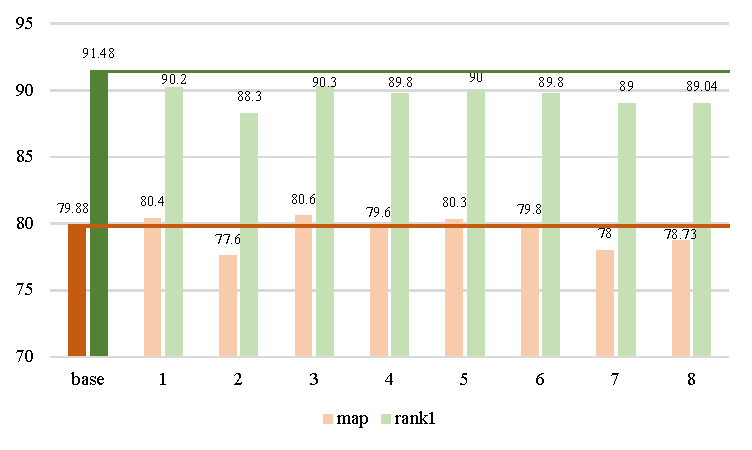
\includegraphics[width=\linewidth]{figs/pdf/samepose.pdf}
\caption{ReID results with images generated with the same pose on Market1501.}
\label{fig:samepose}
\end{figure}

\begin{figure}
\centering
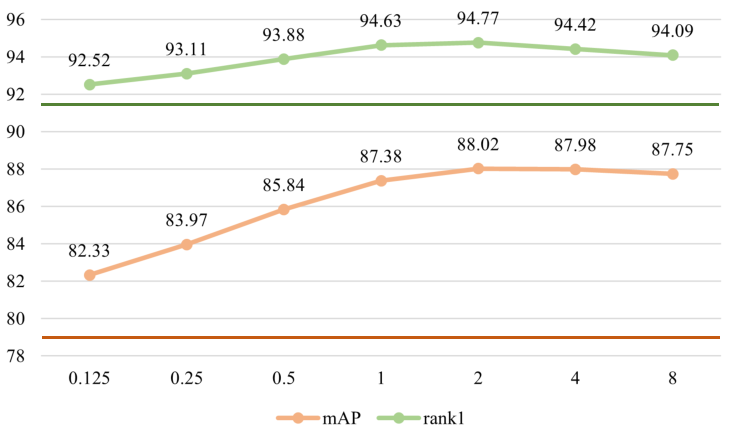
\includegraphics[width=0.9\linewidth]{figs/pdf/eta.pdf}
\caption{Impact of the quality coefficient \( \eta \) with TransReID on Market1501. The dark color lines are the baseline.}
\label{fig:eta}
\end{figure}

\begin{figure}
\centering
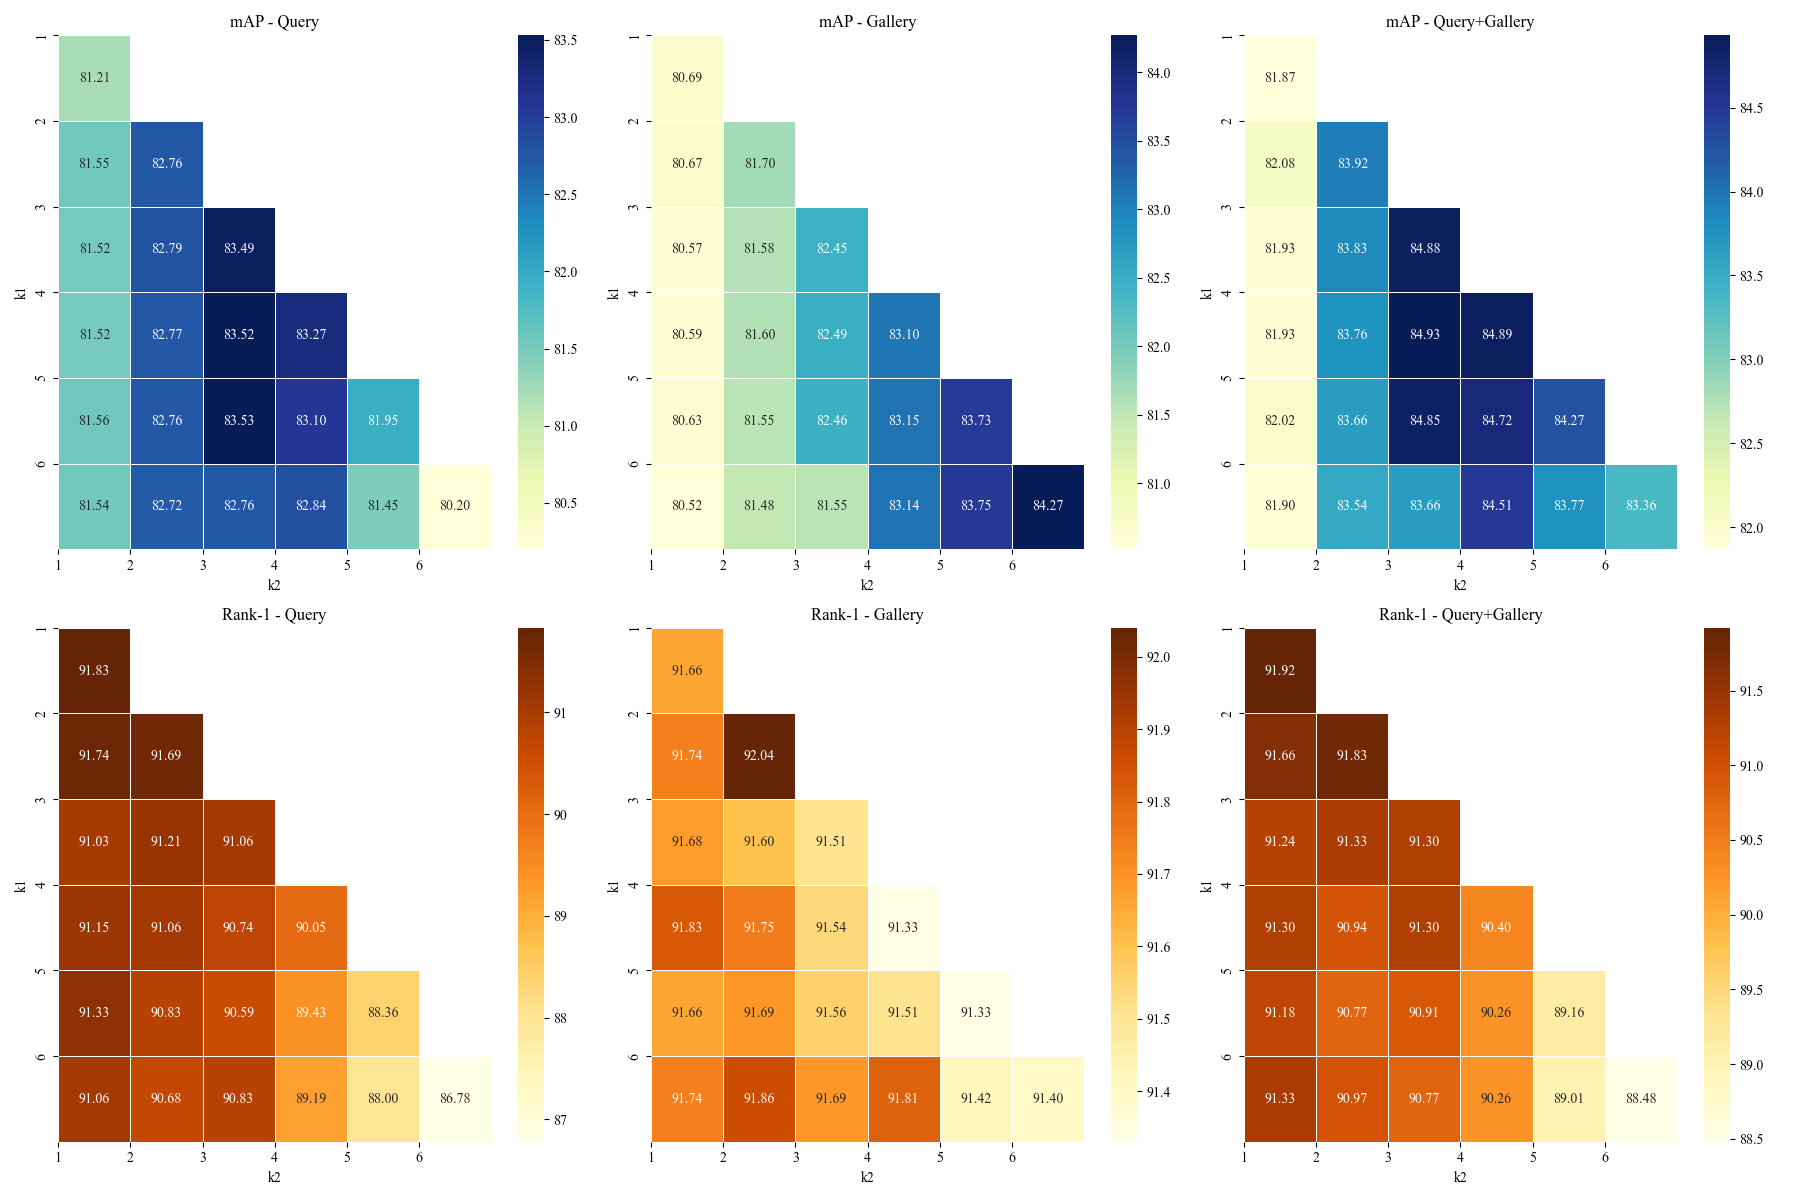
\includegraphics[width=0.9\linewidth]{figs/k1k2.png}
\caption{$k_1/k_2$ analysis of Neighbor Feature Centralization (NFC) with TransReID on Market1501 without re-ranking.}
\label{fig:k1k2}
\end{figure}

\section{Experiments Supplementary}
\begin{figure*}
\centering
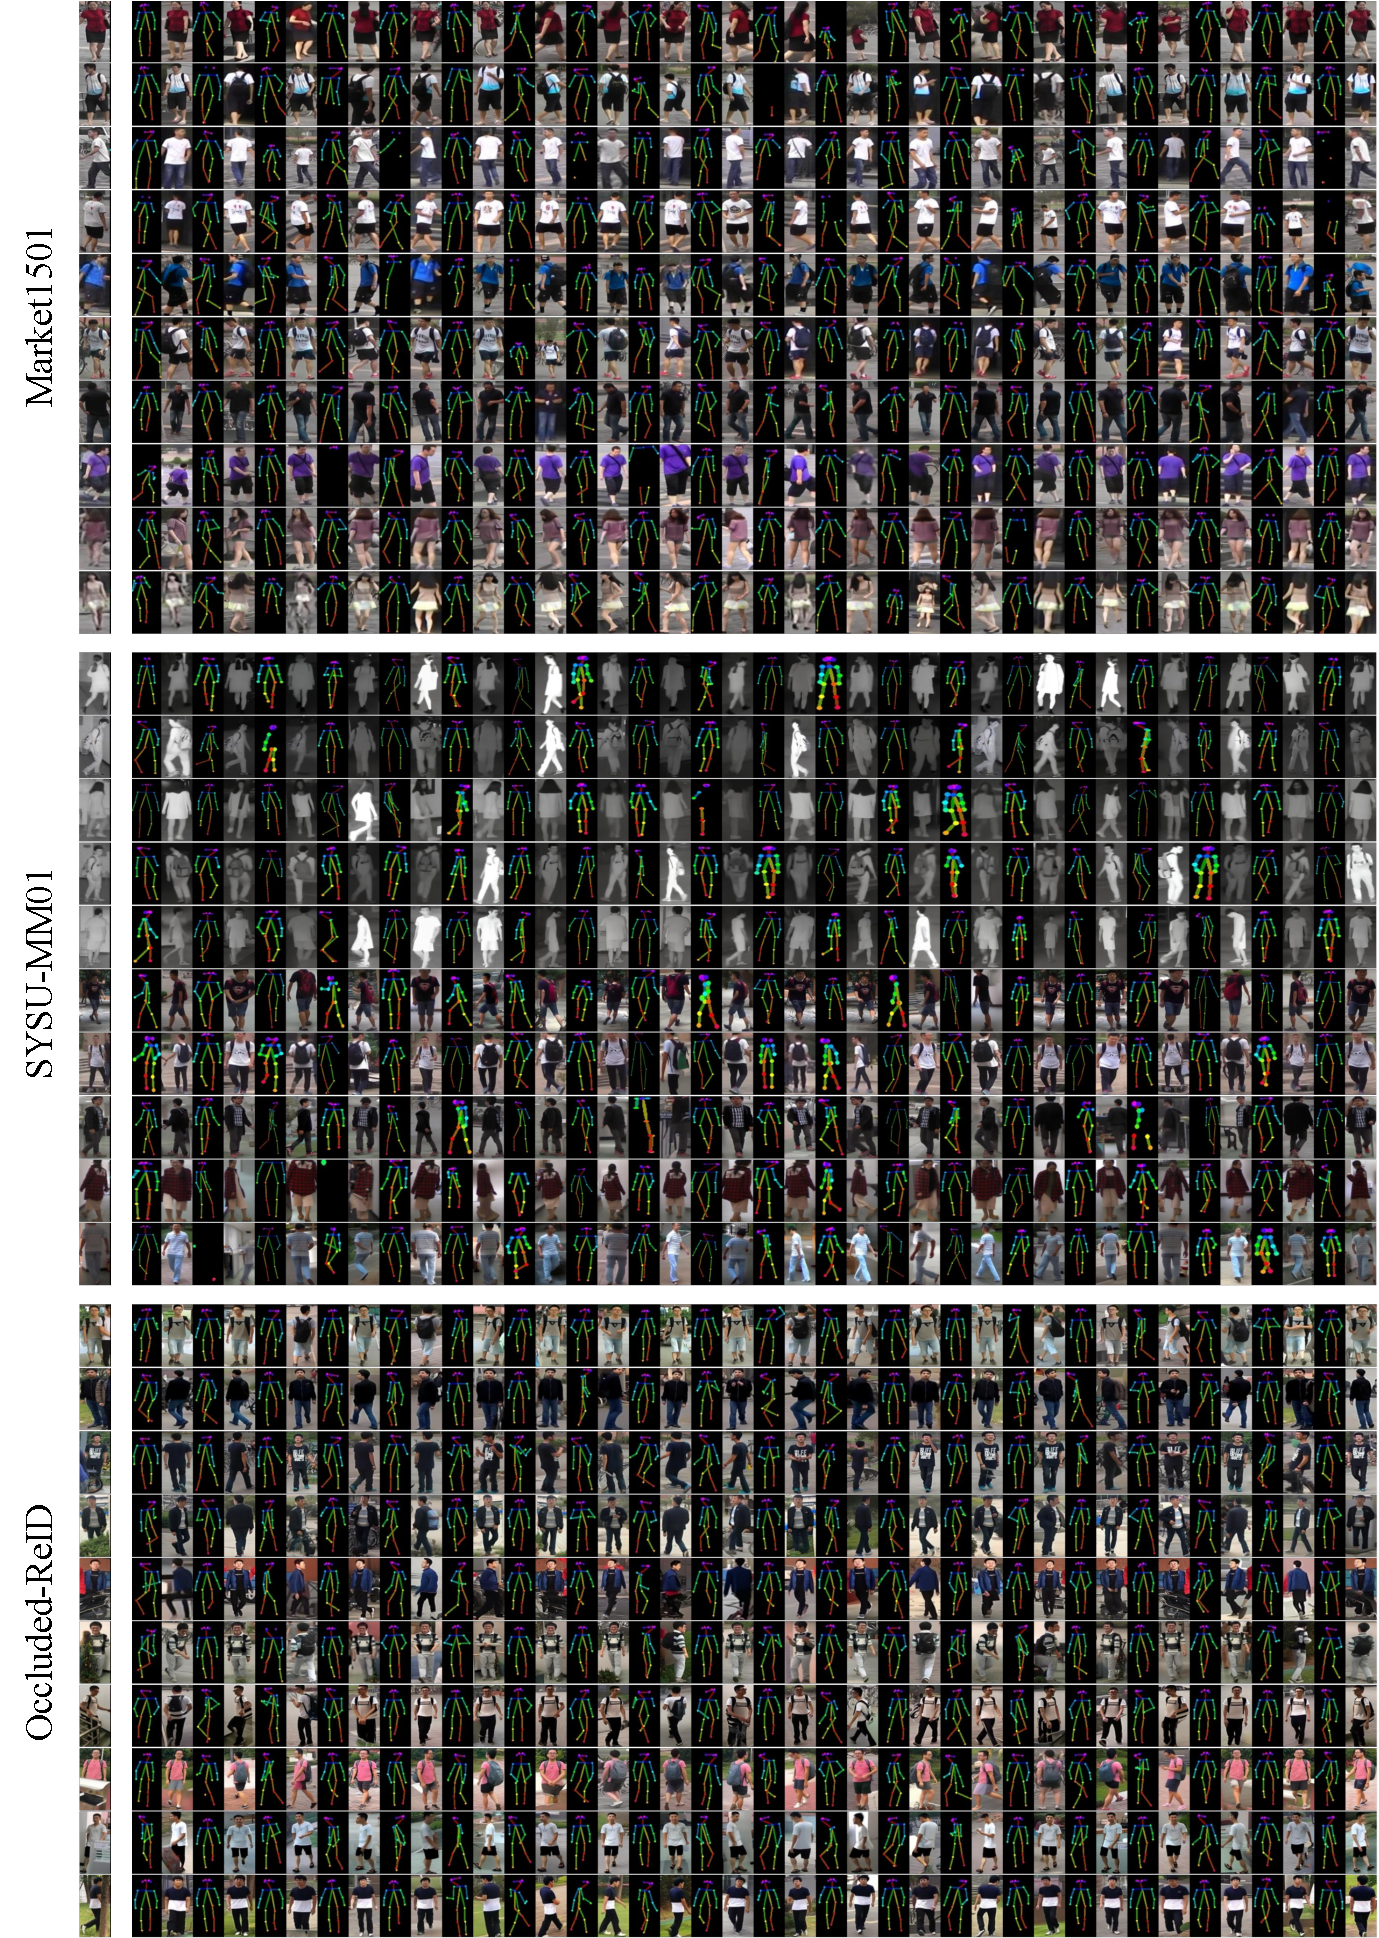
\includegraphics[width=\linewidth]{figs/pdf/random_l.pdf}
\caption{More random generated images on three datasets.}
\label{fig:random_all}
\end{figure*}
\subsection{Data Cleansing}
Training an effective generative model requires high-quality data support. In current ReID (Person Re-Identification) datasets, there are many low-quality images, and removing them can help reduce interference to the model. In our experiments, we found two main issues that need to be addressed: \textbf{Extremely Low-quality Images}: The dataset contains images with such low resolution that even the human eye cannot recognize them as a "person". \textbf{Pose Estimation Failures}: The pose estimation model inevitably fails to detect pedestrian poses in some images.

\subsubsection{Extremely Low-quality Images}

To address this, manual filtering is impractical. Therefore, we designed an automated filtering algorithm. We leverage normal distribution of feature vector, if the feature on the edge of the distribution, largely due to the data itself is out of the distribution of its identity, and it can be picked up. 
% We calculate the mean and covariance matrix of the feature vectors for each ID and filter out samples whose feature distances lie outside a predefined quantile range.

Let \( \mathbf{f}_i \in \mathbb{R}^d \) denote the feature vector of the \( i \)-th sample of a particular identity, where \( d \) is the feature dimension. The mean vector \( \boldsymbol{\mu} \) and covariance matrix \( \boldsymbol{\Sigma} \) are computed as follows:
\begin{equation} 
\boldsymbol{\mu} = \frac{1}{N} \sum_{i=1}^{N} \mathbf{f}_i, \quad \boldsymbol{\Sigma} = \frac{1}{N} \sum_{i=1}^{N} (\mathbf{f}_i - \boldsymbol{\mu})(\mathbf{f}_i - \boldsymbol{\mu})^\top
\end{equation}
where \( N \) is the number of samples for a given ID.

To detect outliers, we compute the Mahalanobis distance \( d_i \) of each feature vector \( \mathbf{f}_i \) from the mean vector \( \boldsymbol{\mu} \), defined as:
\begin{equation}
dis_i = \sqrt{ (\mathbf{f}_i - \boldsymbol{\mu})^\top \boldsymbol{\Sigma}^{-1} (\mathbf{f}_i - \boldsymbol{\mu}) }
\end{equation}

Given that the feature vectors are assumed to follow a multivariate normal distribution, we use quantiles of the Mahalanobis distance to filter out outliers. Specifically, we define a lower bound \( Q_p \) and an upper bound \( Q_{1-p} \) based on the \( p \)-th and \( (1 - p) \)-th quantiles, respectively. Samples with distances outside this range are considered outliers and are removed, and can get a set $S^{\text{ref}}_{i}$ for $i^{th}$ ID:
\begin{equation} \label{outliers}
S_i^{\text{ref}} = \{ \mathbf{x}_i \mid dis_i \in [Q_p, Q_{1-p}] \}
\end{equation}



\begin{figure}
\centering
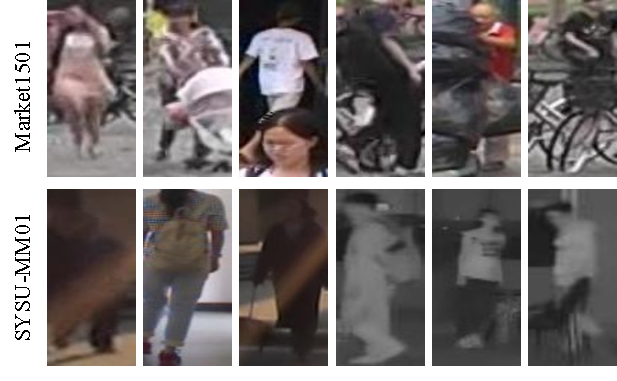
\includegraphics[width=0.8\linewidth]{figs/pdf/outliers.pdf}
\caption{Some outliers detected via the mechanism formulated as Equation.\ref{outliers} on Market1501 and SYSU-MM01 with quartile 0.005.}
\label{fig:outliers}
\end{figure}


\subsubsection{Pose Filtering for 'Failed' Pose Estimation}
\label{PoseValid}
We designed a pose filtering algorithm called PoseValid to eliminate cases where pose extraction has "completely failed." This algorithm checks the validity of the pose keypoints based on factors such as occlusion, keypoint positions, angles, and limb proportions, then get the set of valid poses.
\begin{equation}
S^{\text{trg}}_i = \{ \mathbf{x}_i \mid \text{PoseValid}(\mathbf{x}_i) \text{ and } dis_i \in [Q_p, Q_{1-p}] \}
\end{equation}
where the pose detector in this paper uses pretrained model of DWpose\cite{yang2023effective}. Given a set of keypoints representing a pose, we normalize the pose using the following steps:
\begin{enumerate}
    \item Compute the body height ($h$):\\
    Calculate the Euclidean distance between the Neck (keypoint 1) and the Left Hip (keypoint 11):
    \[
    h = \left\| \mathbf{k}_{\text{Neck}} - \mathbf{k}_{\text{LHip}} \right\|
    \]
    \item Translate the pose:\\
    Shift all keypoints so that the Neck is at the origin:
    \[
    \mathbf{k}'_i = \mathbf{k}_i - \mathbf{k}_{\text{Neck}}
    \]
    \item Scale the pose:\\
    Divide each keypoint by the body height to normalize the size:
    \[
    \mathbf{k}^{\text{normalized}}_i = \frac{\mathbf{k}'_i}{h}
    \]
\end{enumerate}
Then, the filtering process of PoseValid function evaluates the validity of pose keypoints by applying constraints on limb lengths, symmetry, and keypoint positions. 

\subsection{Generation quality and Pose Representation Study}
To assess the quality of the generated images, we replaced the real images in the dataset with images of the same pose and performed inference validation. The results, as shown in Fig.\ref{fig:samepose}, indicate that the original model still successfully matches pedestrians without significant performance degradation. Even with all images in the same pose, the model can effectively differentiate between individuals. This suggests that our generated images are of high quality, retaining the main characteristics of the original images without notably impacting the ReID model. Moreover, we found that pedestrians walking at an angle have higher distinguishability compared to other poses (front, back, and side views), which are more representative of their identities.


\begin{table}[]
\small
\renewcommand{\arraystretch}{1.0}
\renewcommand\tabcolsep{5pt}
\centering
    \begin{tabular}{cc|ccc}
        \hline
        +Ours & +Rerank & mAP & Rank1  \\ \hline
        \ding{55} &\ding{55} & 79.88 & 91.48 \\
        \ding{55} &\ding{51} & 89.56 & 92.07  \\ \hline
        \rowcolor{gray!20}
        \ding{51} &\ding{55} &90.39&94.74\\
        \rowcolor{gray!20}
        \ding{51} &\ding{51}  & \textbf{92.79}&	\textbf{94.83} \\ \hline
    \end{tabular}
    \caption{Compared to k-reciprocal rerank with official settings on Market1501 ($k_1$=20,$k_2$=6).}
    \label{tab:rerank}
\end{table}

\begin{table}[]
\small
\renewcommand{\arraystretch}{1.0}
\renewcommand\tabcolsep{5pt}
\centering
        \begin{tabular}{c|ccc}
        \hline
        Methods & mAP & Rank1  \\ \hline
        TransReID on MSMT17 & 67.80	&85.33\\
        \rowcolor{gray!20}
        +ours & 74.06	&86.55	  \\ \hline
    \end{tabular}
    \caption{Experiment on MSMT17 with TransReID and their official weights.}
    \label{tab:more}
\end{table}


\subsection{More Random Generation}
We provide additional randomly generated images in Fig.\ref{fig:random_all} from Market-1501, SYSU-MM01 and Occluded-ReID datasets.


\subsection{Collaborate with Re-ranking}
Since our method does not change the features' original distribution,
it could collaborate post-processing strategies like rerank, as shown in Tab.\ref{tab:rerank}.

\subsection{Results on MSMT17 with TransReID}
We conduct a simple experiment on MSMT17 dataset with with TransReID and their official pre-trained weights. As shown in Tab.\ref{tab:more}.

\subsection{Comparisons with state-of-the-art methods on three ReID benchmarks}
Comparison on three ReID benchmarks. Since Our method can be applied to any baseline, we choose three methods from three benchmarks which have the official codes and pre-trained weights. With our method, we achieve the new SOTA in three benchmarks, as shown in Fig.\ref{tab:sota_m} and Fig.\ref{tab:sys}.



\begin{table}
\centering
\renewcommand\tabcolsep{5pt}

\begin{tabular}{c|cc|cc}
\hline
 \multirow{2}{*}{Methods}& \multicolumn{2}{c|}{Market1501} & \multicolumn{2}{c}{Occluded-reID} \\ \cline{2-5}
 & Rank-1 & mAP & Rank-1  & mAP \\
\hline
BoT\cite{luo2019bag} & 94.5 & 85.9 & 58.4 & 52.3 \\
PCB\cite{sun2018beyond}& 93.8 & 81.6& - & - \\
VGTri\cite{yang2021learning} & - & - & 81.0 & 71.0 \\
PVPM\cite{gao2020pose} & - & - & 66.8 & 59.5 \\
HOReID\cite{wang2020high} & 94.2 & 84.9 & 80.3 & 70.2 \\
ISP\cite{zhu2020identity} & 95.3 & 88.6 & - & -\\
PAT\cite{li2021diverse} & 95.4 & 88.0 & 81.6 & 72.1 \\
TRANS\cite{he2021transreid} & 95.2 & 88.9 & - & - \\
CLIP\cite{li2023clip} & 95.7 & 89.8 & - & - \\
SOLIDER\cite{chen2023beyond} & 96.9 & 93.9 & - & - \\
SSGR\cite{yan2021occluded} & 96.1 & 89.3 & 78.5 & 72.9 \\
FED\cite{wang2022feature} & 95.0 & 86.3& 86.3 & 79.3 \\
BPBreid\cite{somers2023body} & 95.7 & 89.4 & 82.9 & 75.2\\
PFD\cite{wang2022pose} & 95.5 & 89.7 & 83.0 & 81.5 \\
KPR\textsubscript{IN}\cite{somers2025keypoint} & 95.9 & 89.6 & 85.4 & 79.1 \\
KPR\textsubscript{SOL}\cite{somers2025keypoint} & 96.62 &93.22 &84.83& 82.6\\
\hline
\rowcolor{gray!20}
CLIP+ours & 97.3 & 94.9 & - & -\\
\rowcolor{gray!20}
KPR\textsubscript{IN}+ours & - & - & 91 & 89.34 \\
\hline
\end{tabular}
\caption{Comparisons with state-of-the-art methods on Market1501 and Occluded-reID.}
\label{tab:sota_m}
\end{table}
\begin{table}
\small
\centering
% \renewcommand{\arraystretch}{1.1}
\renewcommand\tabcolsep{5pt}
	\begin{tabular}{l|cc|cc}
		\hline
		\multirow{2}{*}{Methods} & \multicolumn{2}{c|}{All-Search} &\multicolumn{2}{c}{Indoor-Search}\\ \cline{2-5}
              & mAP & Rank-1 & mAP & Rank-1 \\ \cline{1-5}
             PMT\cite{lu2023learning}& 66.13& 67.70& 77.81& 72.95\\
             MCLNet~\cite{hao2021cross}& 61.98 &65.40&76.58 &72.56\\
             MAUM~\cite{Liu2022LearningMU}& 68.79 &71.68& 81.94 &76.9\\
             CAL\cite{CAL}& 71.73 &74.66& 83.68 &79.69\\
             SAAI(w/o AIM)~\cite{fang2023visible}&  71.81& 75.29&  84.6 &81.59\\
             SEFL\cite{feng2023shape}& 72.33 &77.12& 82.95 &82.07\\
             PartMix\cite{kim2023partmix}& 74.62 &77.78& 84.38 &81.52\\
             MID~\cite{Huang2022ModalityAdaptiveMA} & 59.40 &60.27& 70.12 &64.86\\
             FMCNet~\cite{zhang2022fmcnet}& 62.51 &66.34& 74.09 &68.15\\
             MPANet~\cite{wu2021discover}& 68.24 &70.58& 80.95 &76.74\\
             CMT~\cite{jiang2022cross}& 68.57 &71.88& 79.91 &76.90\\
             protoHPE~\cite{zhang2023protohpe}& 70.59 &71.92&81.31 &77.81\\
             MUN~\cite{yu2023modality}& 73.81 &76.24& 82.06 &79.42\\
             MSCLNet~\cite{zhang2022modality}& 71.64 &76.99& 81.17 &78.49\\
             DEEN~\cite{zhang2023diverse}& 71.80 &74.70& 83.30 &80.30\\
             CIFT~\cite{li2022counterfactual}& 74.79 &74.08& 85.61 &81.82\\
             \cline{1-5}
             \rowcolor{gray!20}
            SAAI+ours&76.44&79.33& 86.83& 84.2\\
             \cline{1-5}
	\end{tabular}
             \caption{Comparison with state-of-the-art methods on SYSU-MM01 without re-ranking.}
             \label{tab:sys}                               
\end{table}


% \begin{figure*}
% \centering
% 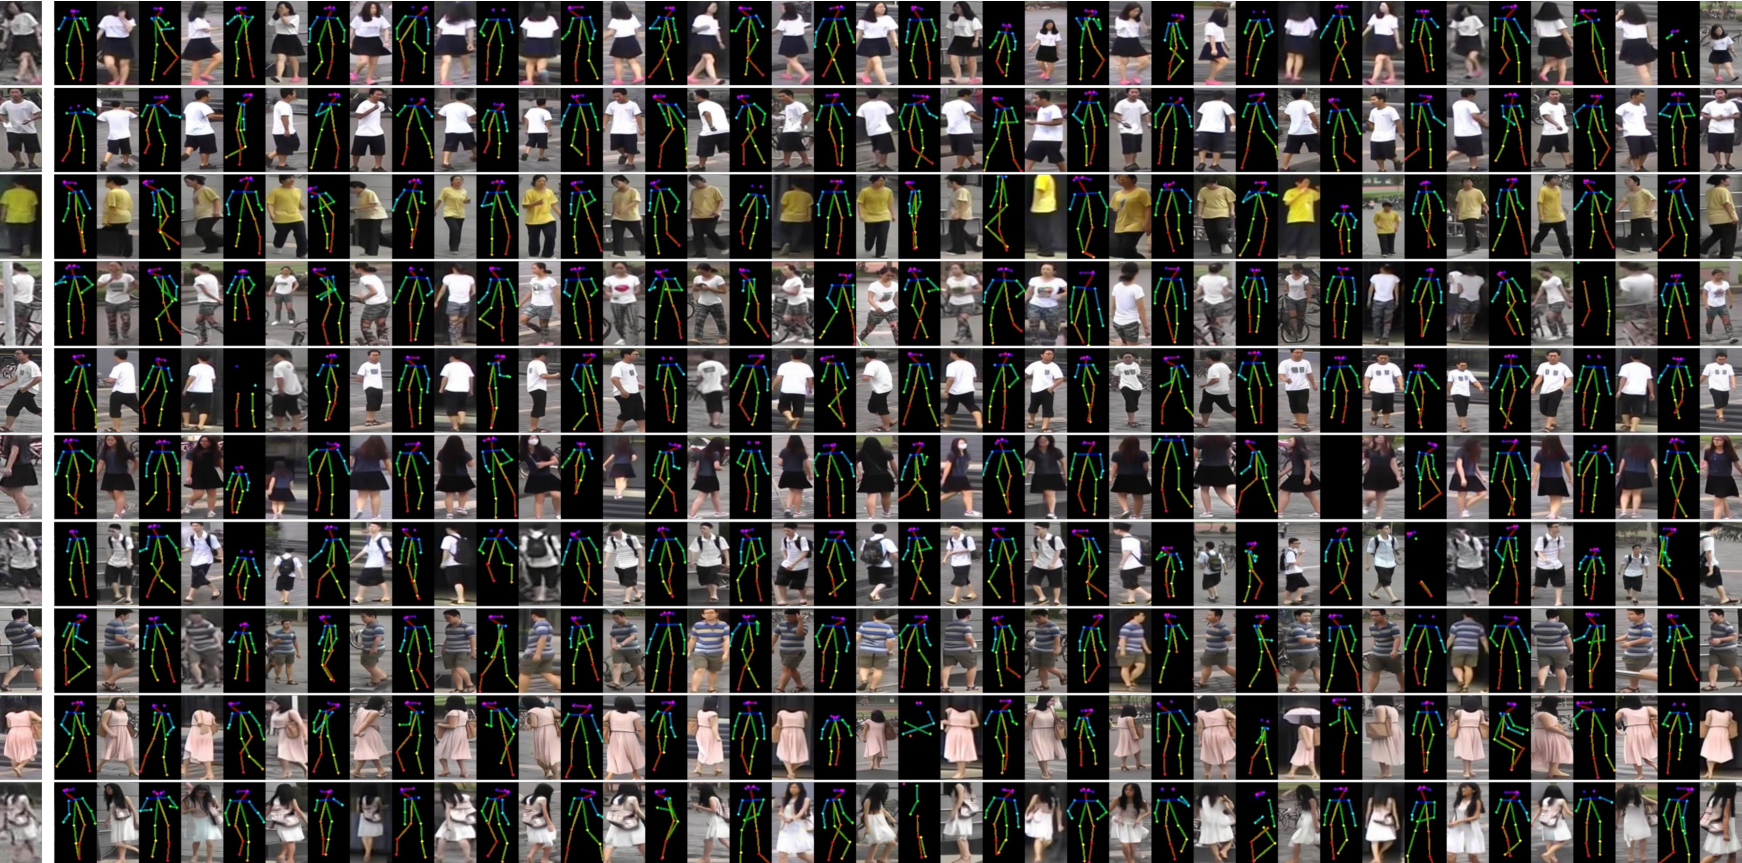
\includegraphics[width=\linewidth]{figs/pdf/random.pdf}
% \caption{Random generated images on Market1501.}
% \label{fig:random_market}
% \end{figure*}

% \begin{figure*}
% \centering
% \includegraphics[width=\linewidth]{figs/pdf/sysu.pdf}
% \caption{Random generated images on SYSU-MM01.}
% \label{fig:random_sysu}
% \end{figure*}


% \begin{figure*}
% \centering
% \includegraphics[width=\linewidth]{figs/pdf/occ.pdf}
% \caption{Random generated images on SYSU-MM01.}
% \label{fig:random_occ}
% \end{figure*}


\subsection{Analysis on quality coefficient $\eta$ of Generation Model}

Fig.\ref{fig:eta} illustrates the effect of adjusting the coefficient $\eta$ on the performance of the ReID model. To evaluate this impact, we gradually increased the value of $\eta$ and observed changes on the mAP and Rank-1 metrics. 

As the value of $\eta$ increases, the performance of the ReID model improves, reaching an optimal point. At $\eta = 2$, both mAP and Rank-1 achieve their maximum values of 88.02\% and 94.77\%, respectively. However, further increasing $\eta$ beyond this point leads to a slight decline in performance. It is easy to find that using generated images to centralize features is effective. However, considering the quality of the generated image, direct adding, although also effective, may not always achieve the best results. Therefore adjusting $\eta$ according to the generation quality of the model in this dataset can better centralize the features.


\subsection{Analysis on $k_1/k_2$ of Neighbor Feature Centralization}
We conducted a detailed analysis of different $k_1$ and $k_2$ combinations, evaluating the results of feature centralization enhancement separately on the Query and Gallery sets, as well as the combined effect (as shown in the Fig.\ref{fig:k1k2}). The selection of these two parameters primarily depends on the number of potential positive samples within the set (adjusting $k_1$) and the confidence in feature associations (adjusting k2). Overall, medium parameter combinations ($k_1$ and $k_2$ in the range of 2-4) provide relatively optimal performance.




























% \begin{equation}
% \mathbf{E}_{i+1} = \text{SiLU}(\text{Conv}_{i, \text{stride}=2}(\text{Conv}_{i}(\mathbf{E}_i)))
% \end{equation}
% \paragraph{Forward Process}

% The Denoising Diffusion Implicit Model (DDIM) \cite{song2020denoising} is fundamental to our approach. The forward process gradually adds Gaussian noise to the data:
% \begin{equation}
% q(\mathbf{z}_t \mid \mathbf{z}_{t-1}) = \mathcal{N}(\mathbf{z}_t; \sqrt{\alpha_t} \mathbf{z}_{t-1}, (1 - \alpha_t) \mathbf{I})
% \end{equation}
% where \( \alpha_t \) controls the noise schedule, and \( \mathbf{z}_t \) is the noisy latent at timestep \( t \).

% \paragraph{Reverse Process}

% The model learns to reverse the diffusion process with classifier-free guidance \cite{ho2022classifier}:
% \begin{equation}
% \begin{aligned}
%     \mathbf{z}_{t-1} &= \boldsymbol{\mu}(\mathbf{z}_t, t, \mathbf{E}_{\text{pose}}, \mathbf{H}) - w \cdot (\hat{\boldsymbol{\epsilon}}^{\text{cond}} - \hat{\boldsymbol{\epsilon}}^{\text{uncond}}) \\
%     \hat{\boldsymbol{\epsilon}}^{\text{cond}} &= \boldsymbol{\epsilon}_{\theta}(\mathbf{z}_t, t, \mathbf{E}_{\text{pose}}, \mathbf{H}) \\
%     \hat{\boldsymbol{\epsilon}}^{\text{uncond}} &= \boldsymbol{\epsilon}_{\theta}(\mathbf{z}_t, t, \mathbf{E}_{\text{pose}}, \mathbf{H} = 0)
% \end{aligned}
% \end{equation}

% The model predicts the mean \( \boldsymbol{\mu} \) of the posterior distribution at each timestep, conditioned on the pose features and conditioning embedding.
% \begin{equation}
% \small
% \boldsymbol{\mu}(\mathbf{z}_t, t, \mathbf{E}_{\text{pose}}, \mathbf{H}) = \frac{1}{\sqrt{\alpha_t}} \left( \mathbf{z}_t - \frac{1 - \alpha_t}{\sqrt{1 - \bar{\alpha}_t}} \boldsymbol{\epsilon}_{\theta}(\mathbf{z}_t, t, \mathbf{E}_{\text{pose}}, \mathbf{H}) \right)
% \end{equation}
% \( \hat{\boldsymbol{\epsilon}} \) is the predicted noise by the denoising UNet, and \( \bar{\alpha}_t = \prod_{s=1}^{t} \alpha_s \).

\end{document}
% \section*{Acknowledgments}
% This work was supported by the National Natural Science Foundation of China (No. 62376016).

\bibliographystyle{assets/plainnat}
\bibliography{paper}

% \clearpage
% \newpage
\beginappendix

\appendix


% \vskip 0.2cm
\section{Experimental Settings}
\label{section:reproduce}

% \vskip -0.2cm
\paragraph{Supervised image classification.} For all supervised classification experiments on ImageNet-1K, we follow the training recipes from ConvNeXt \citep{convnext}.
For ConvNeXt-B and ConvNeXt-L, we use the original hyperparameters without modification.
ViT-B and ViT-L models use the same hyperparameters as ConvNeXt-B, except that for ViT-L, the beta parameters for AdamW are set to (0.9, 0.95), and the stochastic depth rates are set to 0.1 for ViT-B and 0.4 for ViT-L. 

% \vskip 0.2cm
\paragraph{Diffusion models.} We use the official implementation~\citep{dit} for training all DiT models. We find that the default learning rate is suboptimal for the models considered in this paper. To address this, we conduct a simple learning rate search with the LN models and apply the tuned learning rates directly to the DyT models. We also observe that the zero initialization negatively affects the performance of DyT models. Therefore, we retain the zero initialization for LN models but remove the zero initialization for DyT models.

% \vskip 0.2cm
\paragraph{Large Language Models.} In our implementation of LLaMA models~\citep{touvron2023llama, touvron2023llama2, dubey2024llama} with DyT, we introduce an additional learnable scalar parameter immediately after the embedding layer, before any Transformer blocks. We initialize it to the square root of the model embedding dimension $\sqrt{d}$. Without this scaling scalar, we find that the magnitudes of model activations at the beginning of training are too small, and the training struggles to progress. The issue is mitigated by incorporating a learnable scalar, and the model can converge normally. This addition of a scalar is similar to the original Transformer~\citep{vaswani2017attention} design, which uses a fixed scalar of the same value at the same position.

We train all our LLaMA models on the Pile dataset~\citep{pile}. We use the codebase from \texttt{FMS-FSDP} \citep{fms-fsdp}, which provides a default training recipe for the 7B model that closely follows the LLaMA 2 paper~\citep{touvron2023llama2}. We maintain the learning rate at the default 3e-4 for 7B and 13B and 1.5e-4 for 34B and 70B, in line with LLaMA 2.
The batch size is set to 4M tokens
and each model is trained on a total of 200B tokens.


For evaluation, we test the pretrained models on 15 zero-shot commonsense reasoning tasks from \texttt{lm-eval} \citep{eval-harness}: \texttt{anli\_r1}, \texttt{anli\_r2}, \texttt{anli\_r3}, \texttt{arc\_challenge}, \texttt{arc\_easy}, \texttt{boolq}, \texttt{hellaswag}, \texttt{openbookqa}, \texttt{piqa}, \texttt{record}, \texttt{rte}, \texttt{truthfulqa\_mc1}, \texttt{truthfulqa\_mc2}, \texttt{wic}, and \texttt{winogrande}. The selection closely follows that of OpenLLaMA~\citep{openlm2023openllama}. We report the average performance across all tasks.



% \vskip 0.2cm
\paragraph{Self-supervised learning in speech.} For both wav2vec 2.0 models, we retain the first group normalization layer from the original architecture, as it functions primarily as data normalization to handle the unnormalized input data.
We use the official implementation \citep{wav2vec2} without modifying hyperparameters for both the Base and Large models. We report the final validation loss.

% \vskip 0.2cm
\paragraph{Other tasks.} For all other tasks, MAE \citep{he2022masked}, DINO \citep{caron2021emerging}, HyenaDNA \citep{nguyen2024hyenadna} and Caduceus \citep{schiff2024caduceus}, we directly use the publicly released code \citep{mae, dino, hyena, caduceus}, without hyperparameter tuning, for both models with LN and DyT.


% \clearpage
% \newpage
% \vskip -0.2cm
\section{Hyperparameters}
\label{section:tuning}




We present additional experiments to evaluate the impact of hyperparameter tuning, specifically focusing on the learning rate and initialization of $\alpha$ for all non-LLM models. 

\paragraph{Tuning learning rate.} Table~\ref{table:tuned_lr} summarizes performance comparisons between models trained with original versus tuned learning rates. Results indicate that tuning the learning rate provides only modest performance improvements for DyT models. This suggests that the original hyperparameters, initially optimized for LN models, are already well-suited for DyT models. This observation underscores the inherent similarity between the DyT and LN models.

\begin{table}[h]
\centering
\tablestyle{7pt}{1.15}
\begin{tabular}{lcccc}
\toprule
model & LN (original) & DyT (original) & LN (tuned) & DyT (tuned)  \\
\midrule
ViT-B & 82.3\% \scriptsize{(4e-3)} & {82.5\%} \scriptsize{(4e-3)} & - & {82.8\%} \scriptsize{(6e-3)} \\
ViT-L & 83.1\% \scriptsize{(4e-3)} & {83.6\%} \scriptsize{(4e-3)} & - & - \\
ConvNeXt-B & 83.7\% \scriptsize{(4e-3)} & 83.7\% \scriptsize{(4e-3)} & - & - \\
ConvNeXt-L & 84.3\% \scriptsize{(4e-3)} & {84.4\%} \scriptsize{(4e-3)} & - & - \\
\midrule
MAE ViT-B & 83.2\% \scriptsize{(2.4e-3)} & 83.2\% \scriptsize{(2.4e-3)} & - & 83.7\% \scriptsize{(3.2e-3)} \\
MAE ViT-L & {85.5\%} \scriptsize{(2.4e-3)} & 85.4\% \scriptsize{(2.4e-3)} & - & {85.8\%} \scriptsize{(3.2e-3)} \\
DINO ViT-B (patch size 16) & 83.2\% \scriptsize{(7.5e-4)} & {83.4\%} \scriptsize{(7.5e-4)} & 83.3\% \scriptsize{(1e-3)} & - \\
DINO ViT-B (patch size 8) & 84.1\% \scriptsize{(5e-4)} & {84.5\%} \scriptsize{(5e-4)} & - & - \\
\midrule
DiT-B & 64.9 \scriptsize{(4e-4)} & {63.9} \scriptsize{(4e-4)} & - & - \\
DiT-L & {45.9} \scriptsize{(4e-4)} & 45.7 \scriptsize{(4e-4)} & - & - \\
DiT-XL & {19.9} \scriptsize{(4e-4)}  & 20.8 \scriptsize{(4e-4)} & - & - \\
\midrule
wav2vec 2.0 Base & 1.95 \scriptsize{(5e-4)} & 1.95 \scriptsize{(5e-4)} & - & {1.94} \scriptsize{(6e-4)} \\
wav2vec 2.0 Large & 1.92 \scriptsize{(3e-4)} & {1.91} \scriptsize{(3e-4)} & - & - \\
\midrule
HyenaDNA & 85.2\% \scriptsize{(6e-4)} & 85.2\% \scriptsize{(6e-4)} & - & - \\
Caduceus & 86.9\% \scriptsize{(8e-3)} & 86.9\% \scriptsize{(8e-3)} &  - & - \\
\midrule
  \end{tabular}
\caption{\textbf{Performance comparison between original and tuned learning rates for LN and DyT models.} Results show that tuning learning rates provide only modest performance improvements for DyT models, suggesting that the default hyperparameters optimized for LN models are already well-suited for DyT models. Entries marked with ``-'' indicate no performance gain over the original learning rate. The values in parentheses represent the learning rate used. 
}
\label{table:tuned_lr}
\end{table}


\paragraph{Tuning initial value of $\alpha$.} We also investigate the effects of optimizing $\alpha_0$ for DyT models, as presented in Table~\ref{table:tune_alpha}. Findings show only minor performance enhancements for select models when $\alpha_0$ is tuned, indicating that the default initial value ($\alpha_0 = 0.5$) generally achieves near-optimal performance.



\begin{table}[h]
\vskip -0.07in
\centering
\tablestyle{7pt}{1.15}
\begin{tabular}{lcccc}
\toprule
Model & LN  & DyT ($\alpha_0 = 0.5$) & DyT (tuned) \\
\midrule
ViT-B & 82.3\% & 82.5\% & 82.6\% \scriptsize{($\alpha_0 = 1.0$)} \\
ViT-L & 83.1\% & 83.6\% & - \\
ConvNeXt-B & 83.7\% & 83.7\% & - \\
ConvNeXt-L & 84.3\% & 84.4\% & - \\
\midrule
MAE ViT-B & 83.2\% & 83.2\% & 83.4\% \scriptsize{($\alpha_0 = 1.0$)} \\
MAE ViT-L & 85.5\% & 85.4\% & - \\
DINO ViT-B (patch 16) & 83.2\% & 83.4\% & - \\
DINO ViT-B (patch 8) & 84.1\% & 84.5\% & - \\
\midrule
DiT-B & 64.9 & 63.9 & - \\
DiT-L & 45.9 & 45.7 & - \\
DiT-XL & 19.9 & 20.8 & -  \\
\midrule
wav2vec 2.0 Base & 1.95 & 1.95 & - \\
wav2vec 2.0 Large & 1.92 & 1.91 & 1.90 \scriptsize{($\alpha_0 = 1.0$)} \\
\midrule
HyenaDNA & 85.2\% & 85.2\% & -  \\
Caduceus & 86.9\% & 86.9\% & - \\
\midrule
  \end{tabular}
 \caption{\textbf{Impact of tuning the $\alpha_0$ in DyT models.} Optimizing $\alpha_0$ from the default value ($\alpha_0 = 0.5$)  yields only minor performance gains for select DyT models, implying the default initialization already achieves near-optimal performance. Entries marked with ``-'' indicate no improvement over the default $\alpha_0$.
}
\label{table:tune_alpha}
\end{table}








% \clearpage
% \newpage

\section{Replacing Batch Normalization with DyT}
\label{section:batch_normalization}

We investigate the potential of replacing BN with DyT in classic ConvNets such as ResNet-50~\citep{he2016deep} and VGG19~\citep{simonyan2014very}.
Both models are trained on the ImageNet-1K dataset~\citep{deng2009imagenet} using the training recipes provided by \texttt{torchvision}. The DyT models are trained using the same hyperparameters as their BN counterparts.

\begin{table}[h]
\centering
\tablestyle{7pt}{1.15}
\begin{tabular}{lcccccc}
\toprule
model & BN & DyT \\
\midrule
ResNet-50 & 76.2\% & 68.9\% \\
VGG19   & 72.7\% & 71.0\% \\
\midrule
\end{tabular}
\caption{\textbf{ImageNet-1K classification accuracy with BN and DyT.} Replacing BN with DyT in ResNet-50 and VGG19 results in a performance drop, indicating that DyT cannot fully substitute BN in these architectures.}
\label{table:bn_ablation}
\end{table}

The results are summarized in Table~\ref{table:bn_ablation}. Replacing BN with DyT led to a noticeable drop in classification accuracy for both models. These findings indicate that DyT is struggling to fully replace BN in these classic ConvNets. We hypothesize this could be related to BN layers being more frequent in these ConvNets, where they appear once with every weight layer, but LN only appears once per several weight layers in Transformers.

\end{document}